\section{Experiments}
\label{sec:experiments}


\subsection{Experimental Setup}
\label{sec:experimental-setup}

\paragraph{Experimental setup.}
We evaluate on the official 22-task MLE-Bench Lite split released with MLE-Bench unless otherwise stated~\citep{chan2024mlebench}.
Unless specified otherwise, each OpenMLE-Evo configuration is evaluated with three independent runs under a fixed per-task budget of 12 hours on a single RTX 4090 (12 GB VRAM)---a smaller per-task sandbox-compute budget than that used by the vast majority of reported evaluations on MLE-Bench.\footnote{This comparison uses the per-run evaluation compute configurations---accelerator allocation and wall-clock budget---reported in the \href{https://github.com/openai/mle-bench/tree/main/runs\#readme}{official MLE-Bench runs registry}. It does not compare model-inference cost or normalize different accelerators to FLOPs.}
We report three aggregate metrics. \emph{Valid Rate} is the mean number of the 22 tasks for which a run produces a valid submission, written as $x/22$; \emph{Medal Average} is the mean fraction of tasks receiving any Kaggle medal; and \emph{Human Rank} is the fraction of human leaderboard participants whose score is surpassed by the submitted solution, averaged across tasks and runs, so higher is better.
Our primary model is \thirtyfivebmodel{}, which is used for the headline model, system, trajectory, and transfer analyses. We additionally evaluate \thirtybmodel{} as a companion model to test whether the post-training gain reproduces on a second backbone and model scale.


\paragraph{OpenMLE-Evo-Max.}
\openmleevomax{} extends the \openmleevo{} configuration described in Section~\ref{sec:tts-harness} in two ways.
First, it uses a general pipeline to distill reusable cross-task priors from public competition artifacts; all MLE-Bench-related sources are excluded before distillation.
Second, it enables asynchronous multi-GPU parallel search while keeping the total sandbox compute budget unchanged, following insights from AIRA$_2$~\citep{hambardzumyan2026aira_2}.

\subsection{Training and Search Gains Compose}
\label{sec:main-results-lite}


\begin{takeaway}
Under the identical \openmleevo{} harness, execution-grounded post-training
improves the Medal Average of our primary \thirtyfivebmodel{} over its
corresponding Qwen3.6 backbone by $21.22$ percentage points; the companion
\thirtybmodel{} reproduces this gain at $18.18$ percentage points over its
Qwen3 backbone. Combining \thirtyfivebmodel{} with \openmleevomax{} further
reaches $71.21\%$, exceeding GPT-5.5 with Codex by $3.03$ percentage points
and showing that training and search provide complementary improvements.
\end{takeaway}


\begingroup
\definecolor{mainTableGray}{HTML}{F0F2F4}
\definecolor{mainTableCyan}{HTML}{00C1D4}
\definecolor{mainTableMidGray}{HTML}{8C8C8C}
\newcolumntype{M}[1]{>{\raggedright\arraybackslash}p{#1}}
\newcolumntype{N}[1]{>{\centering\arraybackslash}p{#1}}
\newcommand{\mainTablePanel}[1]{%
  \rowcolor{mainTableGray}
  \multicolumn{5}{@{}l@{}}{\rule{0pt}{2.35ex}\textbf{#1}}\\*[-0.15ex]
}
\newcommand{\mainTableGroup}[1]{%
  \multicolumn{5}{@{}l@{}}{%
    \rule{0pt}{2.35ex}%
    \textcolor{mainTableCyan}{\rule{1.6pt}{1.25ex}}\hspace{5pt}%
    \textbf{#1}}\\*[-0.15ex]
}
\newcommand{\mainTableFrontis}[1]{%
  \textcolor{mainTableCyan}{\rule{1.35pt}{1.15ex}}\hspace{4pt}\textbf{#1}}
\newcommand{\mainTableEvoMax}{\textbf{\openmleevomax{}}}
\newcommand{\mainTableBest}[1]{\textbf{#1}}

\small
\setlength{\tabcolsep}{3.2pt}
\renewcommand{\arraystretch}{1.18}
\setlength{\LTpre}{0pt}
\setlength{\LTpost}{0pt}
\setlength{\LTcapwidth}{\linewidth}
\begin{longtable}{@{}M{0.30\linewidth}M{0.22\linewidth}N{0.12\linewidth}N{0.145\linewidth}N{0.125\linewidth}@{}}
\caption{MLE-Bench Lite results. Panel A presents the primary \thirtyfivebmodel{} comparison first, followed by the companion \thirtybmodel{} replication and matched search comparisons; Panels B--C provide broader system context.}
\label{tab:arxiv-main-results}\\[-0.15em]
\toprule
\textbf{Model / system} &
\textbf{Framework} &
\textbf{Valid Rate $\uparrow$} &
\textbf{Medal Average $\uparrow$} &
\textbf{Human Rank $\uparrow$} \\
\midrule
\endfirsthead

\multicolumn{5}{@{}l@{}}{%
  \small\textit{\tablename\ \thetable\ --- continued from previous page}}\\[0.35em]
\toprule
\textbf{Model / system} &
\textbf{Framework} &
\textbf{Valid Rate $\uparrow$} &
\textbf{Medal Average $\uparrow$} &
\textbf{Human Rank $\uparrow$} \\
\midrule
\endhead

\midrule
\multicolumn{5}{r@{}}{%
  \scriptsize\textcolor{mainTableMidGray}{\textit{Continued on next page}}}\\
\endfoot

\bottomrule
\endlastfoot

\mainTablePanel{A. Controlled comparisons}
\mainTableGroup{\thirtyfivebmodel{}}
Qwen3.6-35B-A3B & \openmleevo{} & 19.67/22 & 39.39\% & 0.5828 \\
\rowcolor{mainTableGray}
\mainTableFrontis{\thirtyfivebmodel{}} & \openmleevo{} & 21.67/22 & \frontisThirtyFiveEvoResult{} & \frontisThirtyFiveEvoHumanRank{} \\
\rowcolor{mainTableGray}
\mainTableFrontis{\thirtyfivebmodel{}} & \mainTableEvoMax & 22.00/22 & \mainTableBest{\frontisThirtyFiveEvoMaxResult{}} & \mainTableBest{\frontisThirtyFiveEvoMaxHumanRank{}} \\
\addlinespace[0.45em]

\mainTableGroup{\thirtybmodel{}}
Qwen3-30B-A3B\footnote{The detailed version is Qwen3-30B-A3B-Thinking-2507.} & \openmleevo{} & 17.33/22 & 34.85\% & 0.5573 \\
\textbf{\thirtybmodel{}} & \openmleevo{} & 21.67/22 & \frontisThirtyEvoResult{} & \frontisThirtyEvoHumanRank{} \\
\textbf{\thirtybmodel{}} & \mainTableEvoMax & 22.00/22 & \frontisThirtyEvoMaxResult{} & \frontisThirtyEvoMaxHumanRank{} \\
\addlinespace[0.45em]

\mainTableGroup{Matched harness comparison · GLM-5.2}
GLM-5.2 & Claude Code & 21.00/22 & 59.09\% & 0.7948 \\*
GLM-5.2 & \openmleevo{} & 19.67/22 & 62.12\% & 0.7069 \\*
GLM-5.2 & \mainTableEvoMax & 22.00/22 & \mainTableBest{66.67\%} & \mainTableBest{0.8164} \\
\addlinespace[0.45em]

\mainTableGroup{Matched harness comparison · MiniMax M3}
MiniMax M3 & Codex & 22.00/22 & 54.55\% & 0.7099 \\
MiniMax M3 & \openmleevo{} & 22.00/22 & 59.09\% & 0.7994 \\
MiniMax M3 & \mainTableEvoMax & 22.00/22 & \mainTableBest{65.15\%} & \mainTableBest{0.8007} \\
\addlinespace[0.45em]

\mainTableGroup{Matched harness comparison · Kimi K2.6}
Kimi K2.6 & Claude Code & 18.00/22 & 59.09\% & 0.7062 \\
Kimi K2.6 & \openmleevo{} & 21.67/22 & \mainTableBest{66.67\%} & \mainTableBest{0.7859} \\
\addlinespace[0.45em]

\mainTableGroup{Matched harness comparison · MiniMax M2.7}
MiniMax M2.7 & Claude Code & 18.00/22 & 45.50\% & 0.5547 \\
MiniMax M2.7 & \openmleevo{} & 22.00/22 & \mainTableBest{50.00\%} & \mainTableBest{0.7039} \\
\addlinespace[0.55em]

\mainTablePanel{B. Broader OpenMLE-Evo system context}
Grok-4.5 & \openmleevo{} & 22.00/22 & 65.15\% & 0.8052 \\
LongCat-2.0 & \openmleevo{} & 21.00/22 & 56.06\% & 0.7343 \\
Doubao Seed 2.1 Pro & \openmleevo{} & 20.33/22 & 56.06\% & 0.7170 \\
Qwen3.7 Plus & \openmleevo{} & 21.67/22 & 54.55\% & 0.7234 \\
DeepSeek-V4-Pro & \openmleevo{} & 21.67/22 & 54.55\% & 0.6849 \\
DeepSeek-V4-Flash & \openmleevo{} & 21.33/22 & 51.52\% & 0.6957 \\
GLM-4.7 & \openmleevo{} & 21.33/22 & 51.52\% & 0.6521 \\
MiMo-V2.5-Pro & \openmleevo{} & 17.00/22 & 40.91\% & 0.5213 \\
Step-3.7 Flash & \openmleevo{} & 19.00/22 & 27.27\% & 0.4953 \\
\addlinespace[0.55em]

\mainTablePanel{C. General-purpose coding-agent references}
GPT-5.6 Sol & Codex & 22.00/22 & 72.73\% & 0.8891 \\
Kimi K3 & Claude Code & 22.00/22 & 72.73\% & 0.8574 \\
GPT-5.5 & Codex & 21.00/22 & 68.18\% & 0.7833 \\
Claude Opus 4.8 & Claude Code & 22.00/22 & 63.64\% & 0.8219 \\
Gemini 3.5 Flash & Gemini CLI & 20.00/22 & 63.64\% & 0.7499 \\
Claude Sonnet 5 & Claude Code & 22.00/22 & 59.09\% & 0.7730 \\
Claude Sonnet 4.6 & Claude Code & 22.00/22 & 54.55\% & 0.7670 \\

\end{longtable}
\endgroup


\paragraph{Primary 35B model and system results.}
Under the identical standard \openmleevo{} harness, execution-grounded post-training improves \thirtyfivebmodel{} over its Qwen3.6-35B-A3B base from $39.39\%$ to \frontisThirtyFiveEvoResult{} Medal Average.
Under this common harness, \thirtyfivebmodel{} also outperforms MiniMax M3, Doubao Seed 2.1 Pro, and DeepSeek-V4-Pro, showing that the post-trained model is competitive beyond its base-model comparison.


After injecting MLE-Bench-disjoint cross-task priors and widening parallel tree search through \openmleevomax{}, \thirtyfivebmodel{} reaches \frontisThirtyFiveEvoMaxResult{}, exceeding GLM-5.2 and MiniMax M3 under the same enhanced harness.
The resulting model--harness system also surpasses GPT-5.5 paired with Codex, demonstrating that the training and search gains compose at the system level. To ensure the robustness of these results, we additionally report the mean and standard deviation across three evaluation runs in Appendix~\ref{app:openmle-repeat-evaluation}.

\paragraph{Cross-model replication on 30B.}
We separately apply the same post-training approach to \thirtybmodel{}. Under the identical standard \openmleevo{} harness, it improves over Qwen3-30B-A3B-Thinking-2507 from $34.85\%$ to \frontisThirtyEvoResult{} Medal Average; with \openmleevomax{}, it further reaches \frontisThirtyEvoMaxResult{} Medal Average and \frontisThirtyEvoMaxHumanRank{} Human Rank. This controlled comparison provides supporting evidence that the post-training and search gains are not confined to the primary 35B checkpoint.
\begin{figure}[!t]
\centering
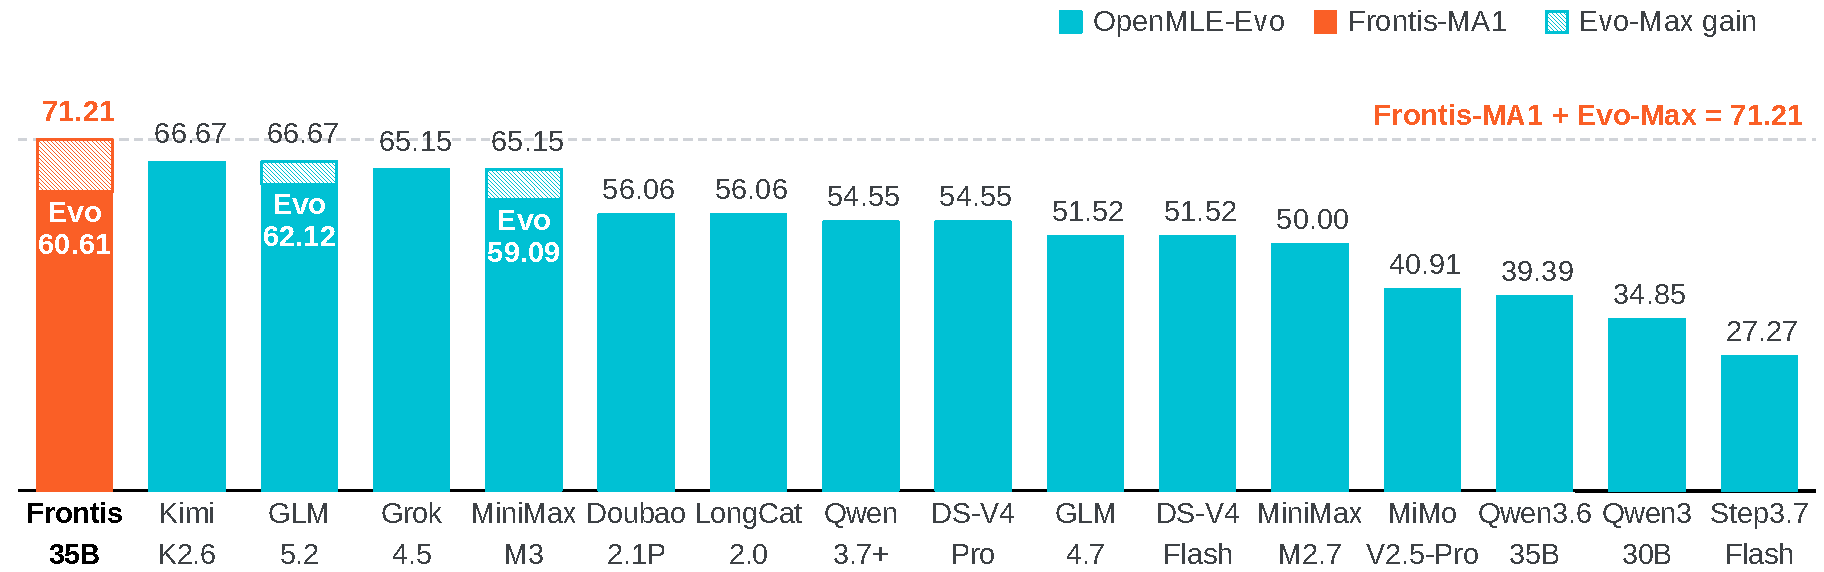
\includegraphics[width=\linewidth]{figures/model_exp.pdf}
\caption{Model performance on MLE-Bench Lite under the common \openmleevo{} harness. Solid bars report standard \openmleevo{} results, while hatched caps show the additional gains from \openmleevomax{} for \thirtyfivebmodel{}, GLM-5.2, and MiniMax M3.}
\label{fig:model-exp}
\end{figure}

\paragraph{Harness gains from domain-specific search.}
\label{sec:harness-comparison}

\begin{figure}[!t]
\centering
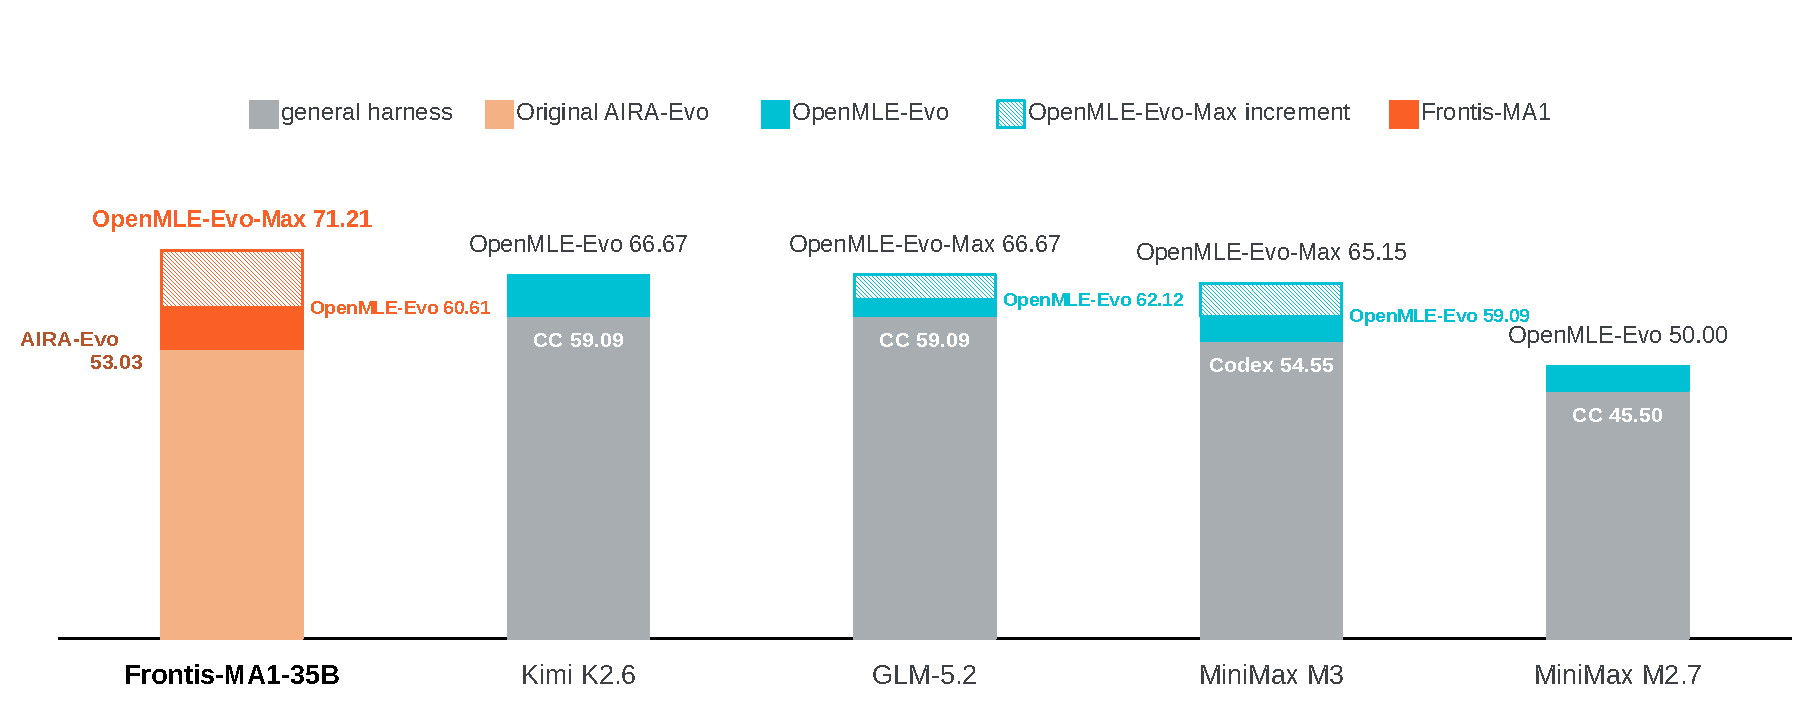
\includegraphics[width=\linewidth]{figures/harness_exp.pdf}
    \caption{Harness comparison on MLE-Bench Lite. Gray reports the general-purpose Claude Code or Codex result, light orange reports original AIRA-Evo for the matched \thirtyfivebmodel{} comparison, cyan reports \openmleevo{}, and hatched caps show the additional \openmleevomax{} gain when available. The OpenMLE model is highlighted in saturated orange.}
\label{fig:harness-exp}
\end{figure}

Figure~\ref{fig:harness-exp} compares harnesses while holding the underlying model fixed.
Across multiple model families, \openmleevo{} consistently converts the same model into a stronger MLE system than general-purpose coding-agent harnesses such as Claude Code and Codex.
Against original AIRA-Evo, the matched \thirtyfivebmodel{} comparison increases Medal Average from $53.03\%$ to \frontisThirtyFiveEvoResult{} under \openmleevo{}.
The consistency of this gain indicates that the improvement comes from search specialized for iterative machine learning engineering, instead of a single favorable model–harness pairing.


\subsection{Long-Horizon Self-Improvement}
\label{sec:search-dynamics-analysis}

\begin{takeaway}
\openmleevo{} continues to improve well beyond the first executable solution. Later \textsc{Improve} and \textsc{Crossover} operations turn accumulated experience into decisive performance gains. This shows that experience-guided long-horizon search converts additional test-time compute into sustained progress rather than redundant sampling.
\end{takeaway}

\textbf{Aggregate long-horizon improvement.}
Figure~\ref{fig:case-study-medal-rate-evolution} shows that combining \thirtyfivebmodel{} with \openmleevomax{} yields sustained improvement throughout long-horizon search. The resulting solutions generalize strongly to the final test, achieving a $71.21\%$ Medal Rate, compared with $68.18\%$ on validation. This performance is comparable to GPT-5.6 Sol with xhigh reasoning and Kimi K3 with their respective harnesses, both of which achieve $72.73\%$ on the final test.

\begin{figure*}[t]
  \centering
  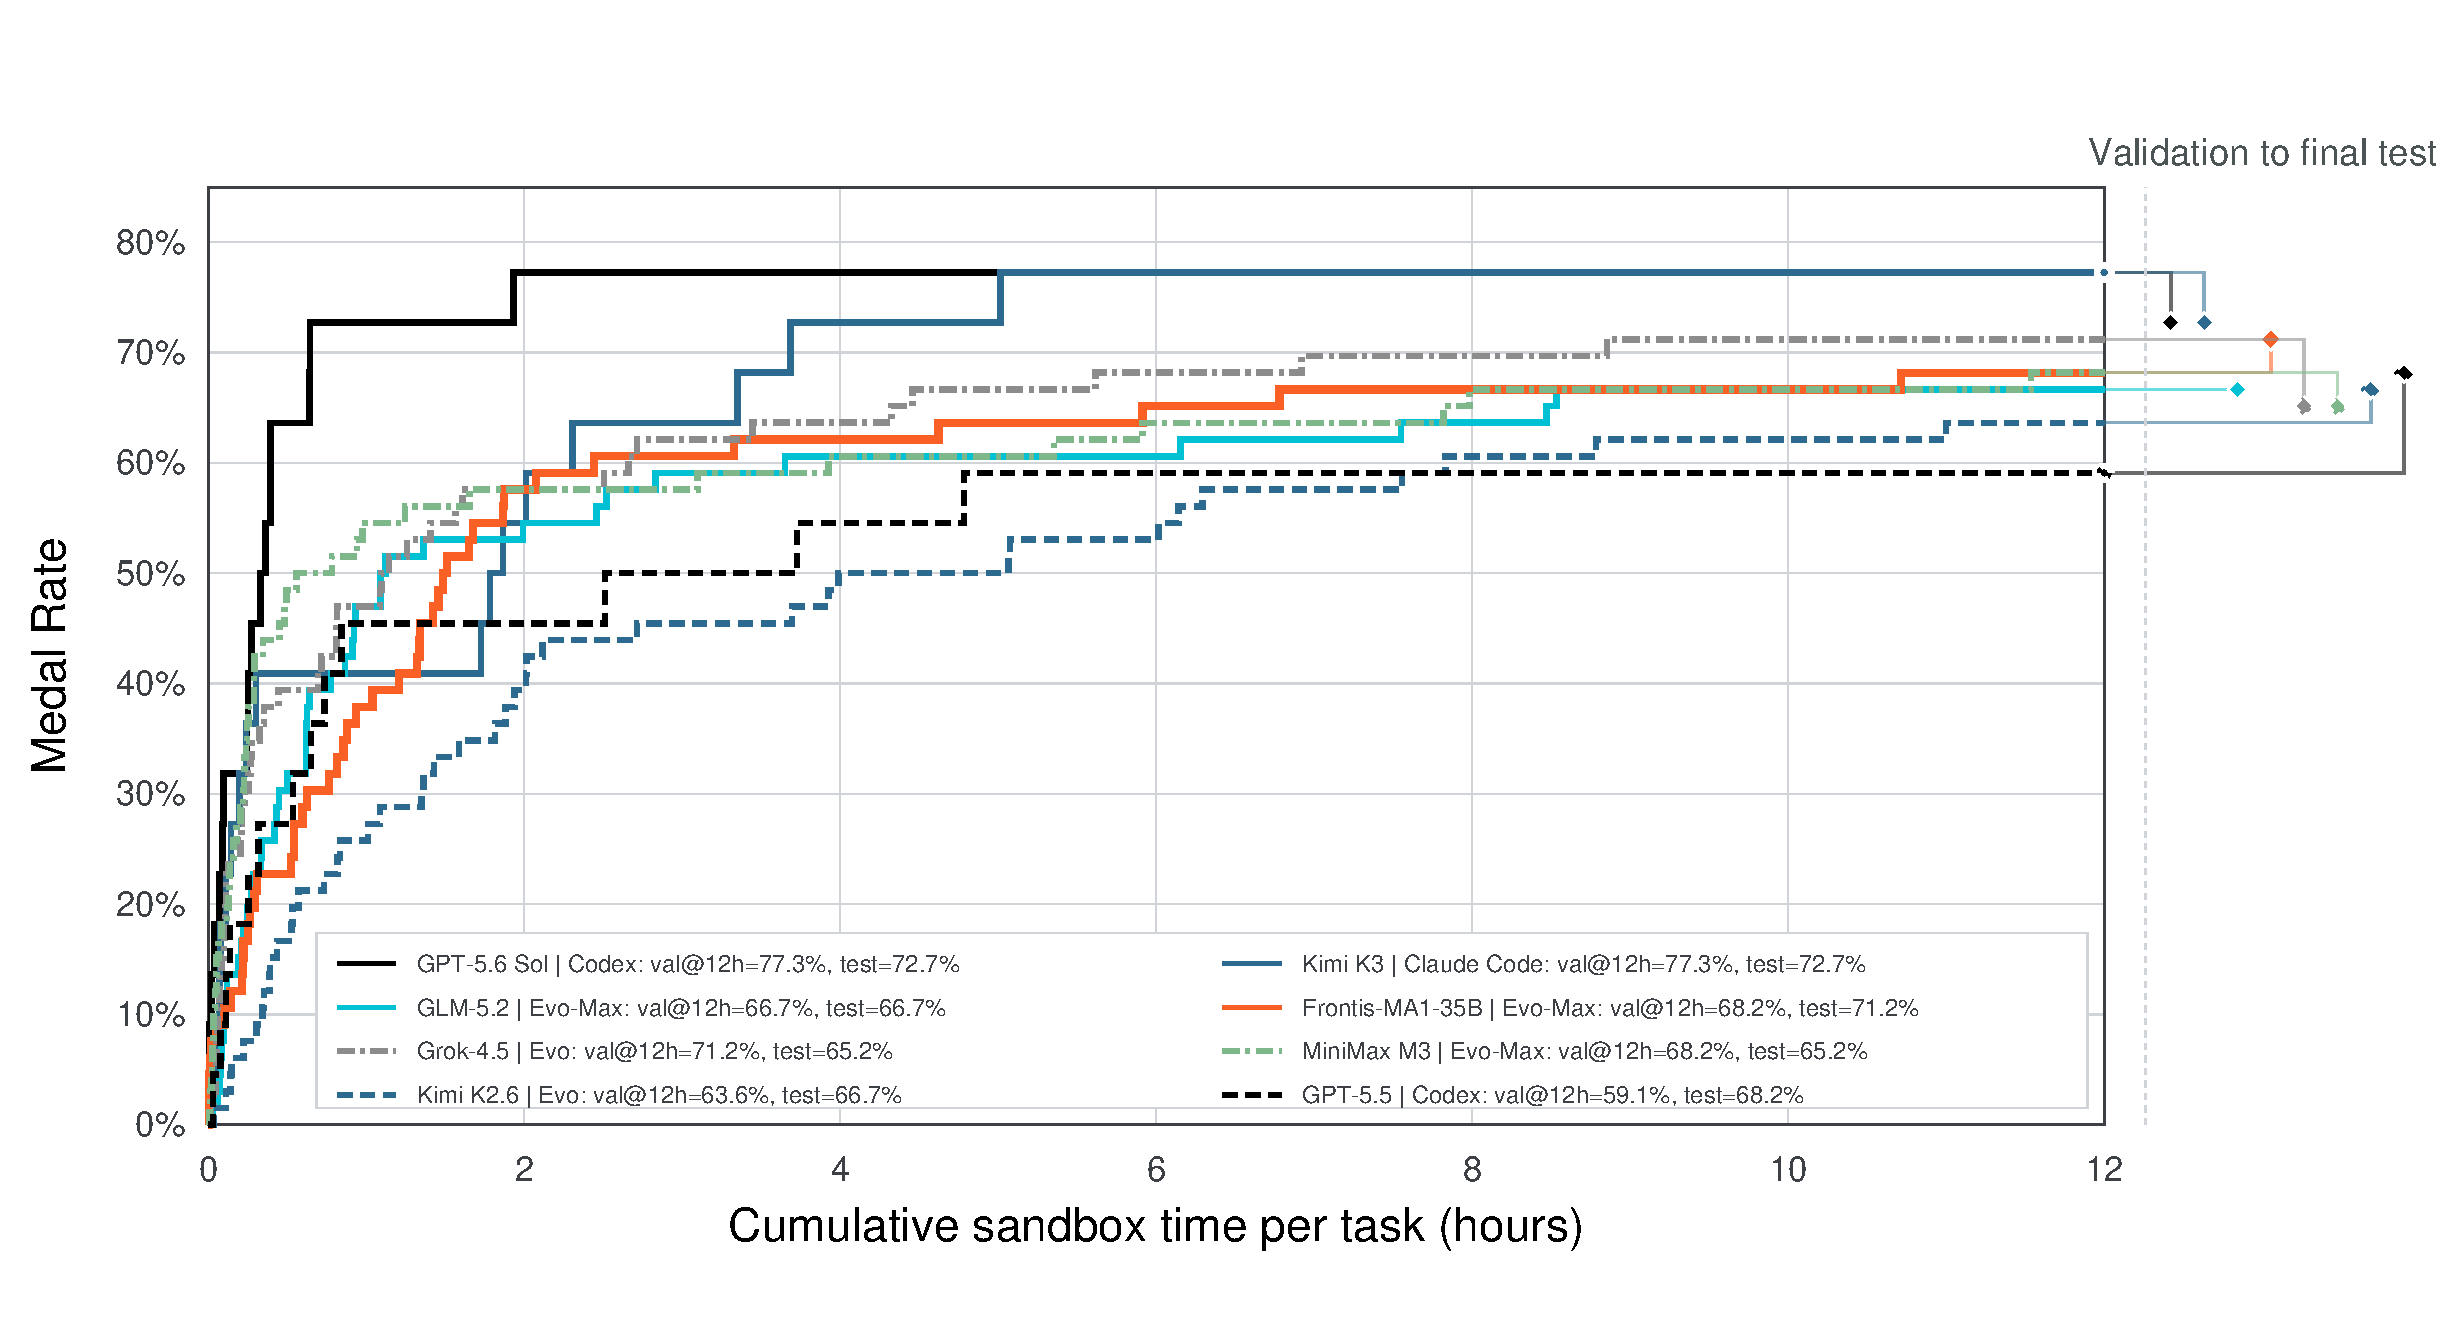
\includegraphics[width=1.0\textwidth]{figures/case_study_human_rank_evolution.pdf}
  \caption{Cross-harness Medal Rate evolution over the 22-task MLE-Bench Lite subset for the top 8 systems. Each step curve reports the fraction of task outcomes whose best-so-far validation score has reached any Kaggle medal by the indicated cumulative sandbox time. The separate final-test panel reports Medal Rate after validation-based node selection, and colored bridges expose the validation-to-test change for each system.}
  \label{fig:case-study-medal-rate-evolution}
\end{figure*}

\textbf{Structured recombination turns additional search into better ML models.}
Figure~\ref{fig:case-study-leaf-late-ops} shows that the main difference is not merely finding an executable solution, but continuing to improve its structure. Under the same \openmleevo{} protocol, the comparison models either plateau at low Human Rank or improve without reaching a medal-quality held-out solution. In contrast, \thirtyfivebmodel{} first uses \textsc{Debug} to establish viable image and tabular branches, then uses \textsc{Crossover} to preserve their complementary evidence and \textsc{Improve} to upgrade the fused model only after that design is stable. These latter operations produce 85.0\% of the total validation gain, indicating that the long horizon is spent accumulating and recombining useful branch evidence, as opposed to repeatedly repairing a single program.
 The resulting trajectory reaches validation Human Rank $0.7713$ and held-out Human Rank $0.9455$ with Bronze; the strongest comparison reaches only $0.6303$ on validation and earns no medal. The lead also holds in the three-epoch averages, making the mechanism less consistent with a single lucky trajectory.


\textbf{Memory-guided recombination breaks the search plateau.}
In figure~\ref{fig:case-study-mlsp-operation-chain}, the comparison trajectories remain near their first viable solutions, whereas \thirtyfivebmodel{} treats submission repair as a starting point and subsequently builds specialized audio branches. Here memory matters through selection, not volume: it preserves which branches contributed robust parsing, imbalance handling, augmentation, and representation quality, while marking an inferior ResNet50 direction as evidence to avoid. \textsc{Improve} and \textsc{Crossover} can therefore combine compatible gains instead of inheriting an undifferentiated history; together they account for $91.9\%$ of the total validation improvement. This produces validation Human Rank $0.7284$ and held-out Human Rank $0.8889$ with Silver, while the strongest comparison reaches only $0.2963$ in validation and none earns a medal. The advantage remains after averaging all three epochs, and the shared corrected prompt rules out the earlier submission-contract ambiguity as its explanation.

\begin{figure}[htbp]
  \centering
  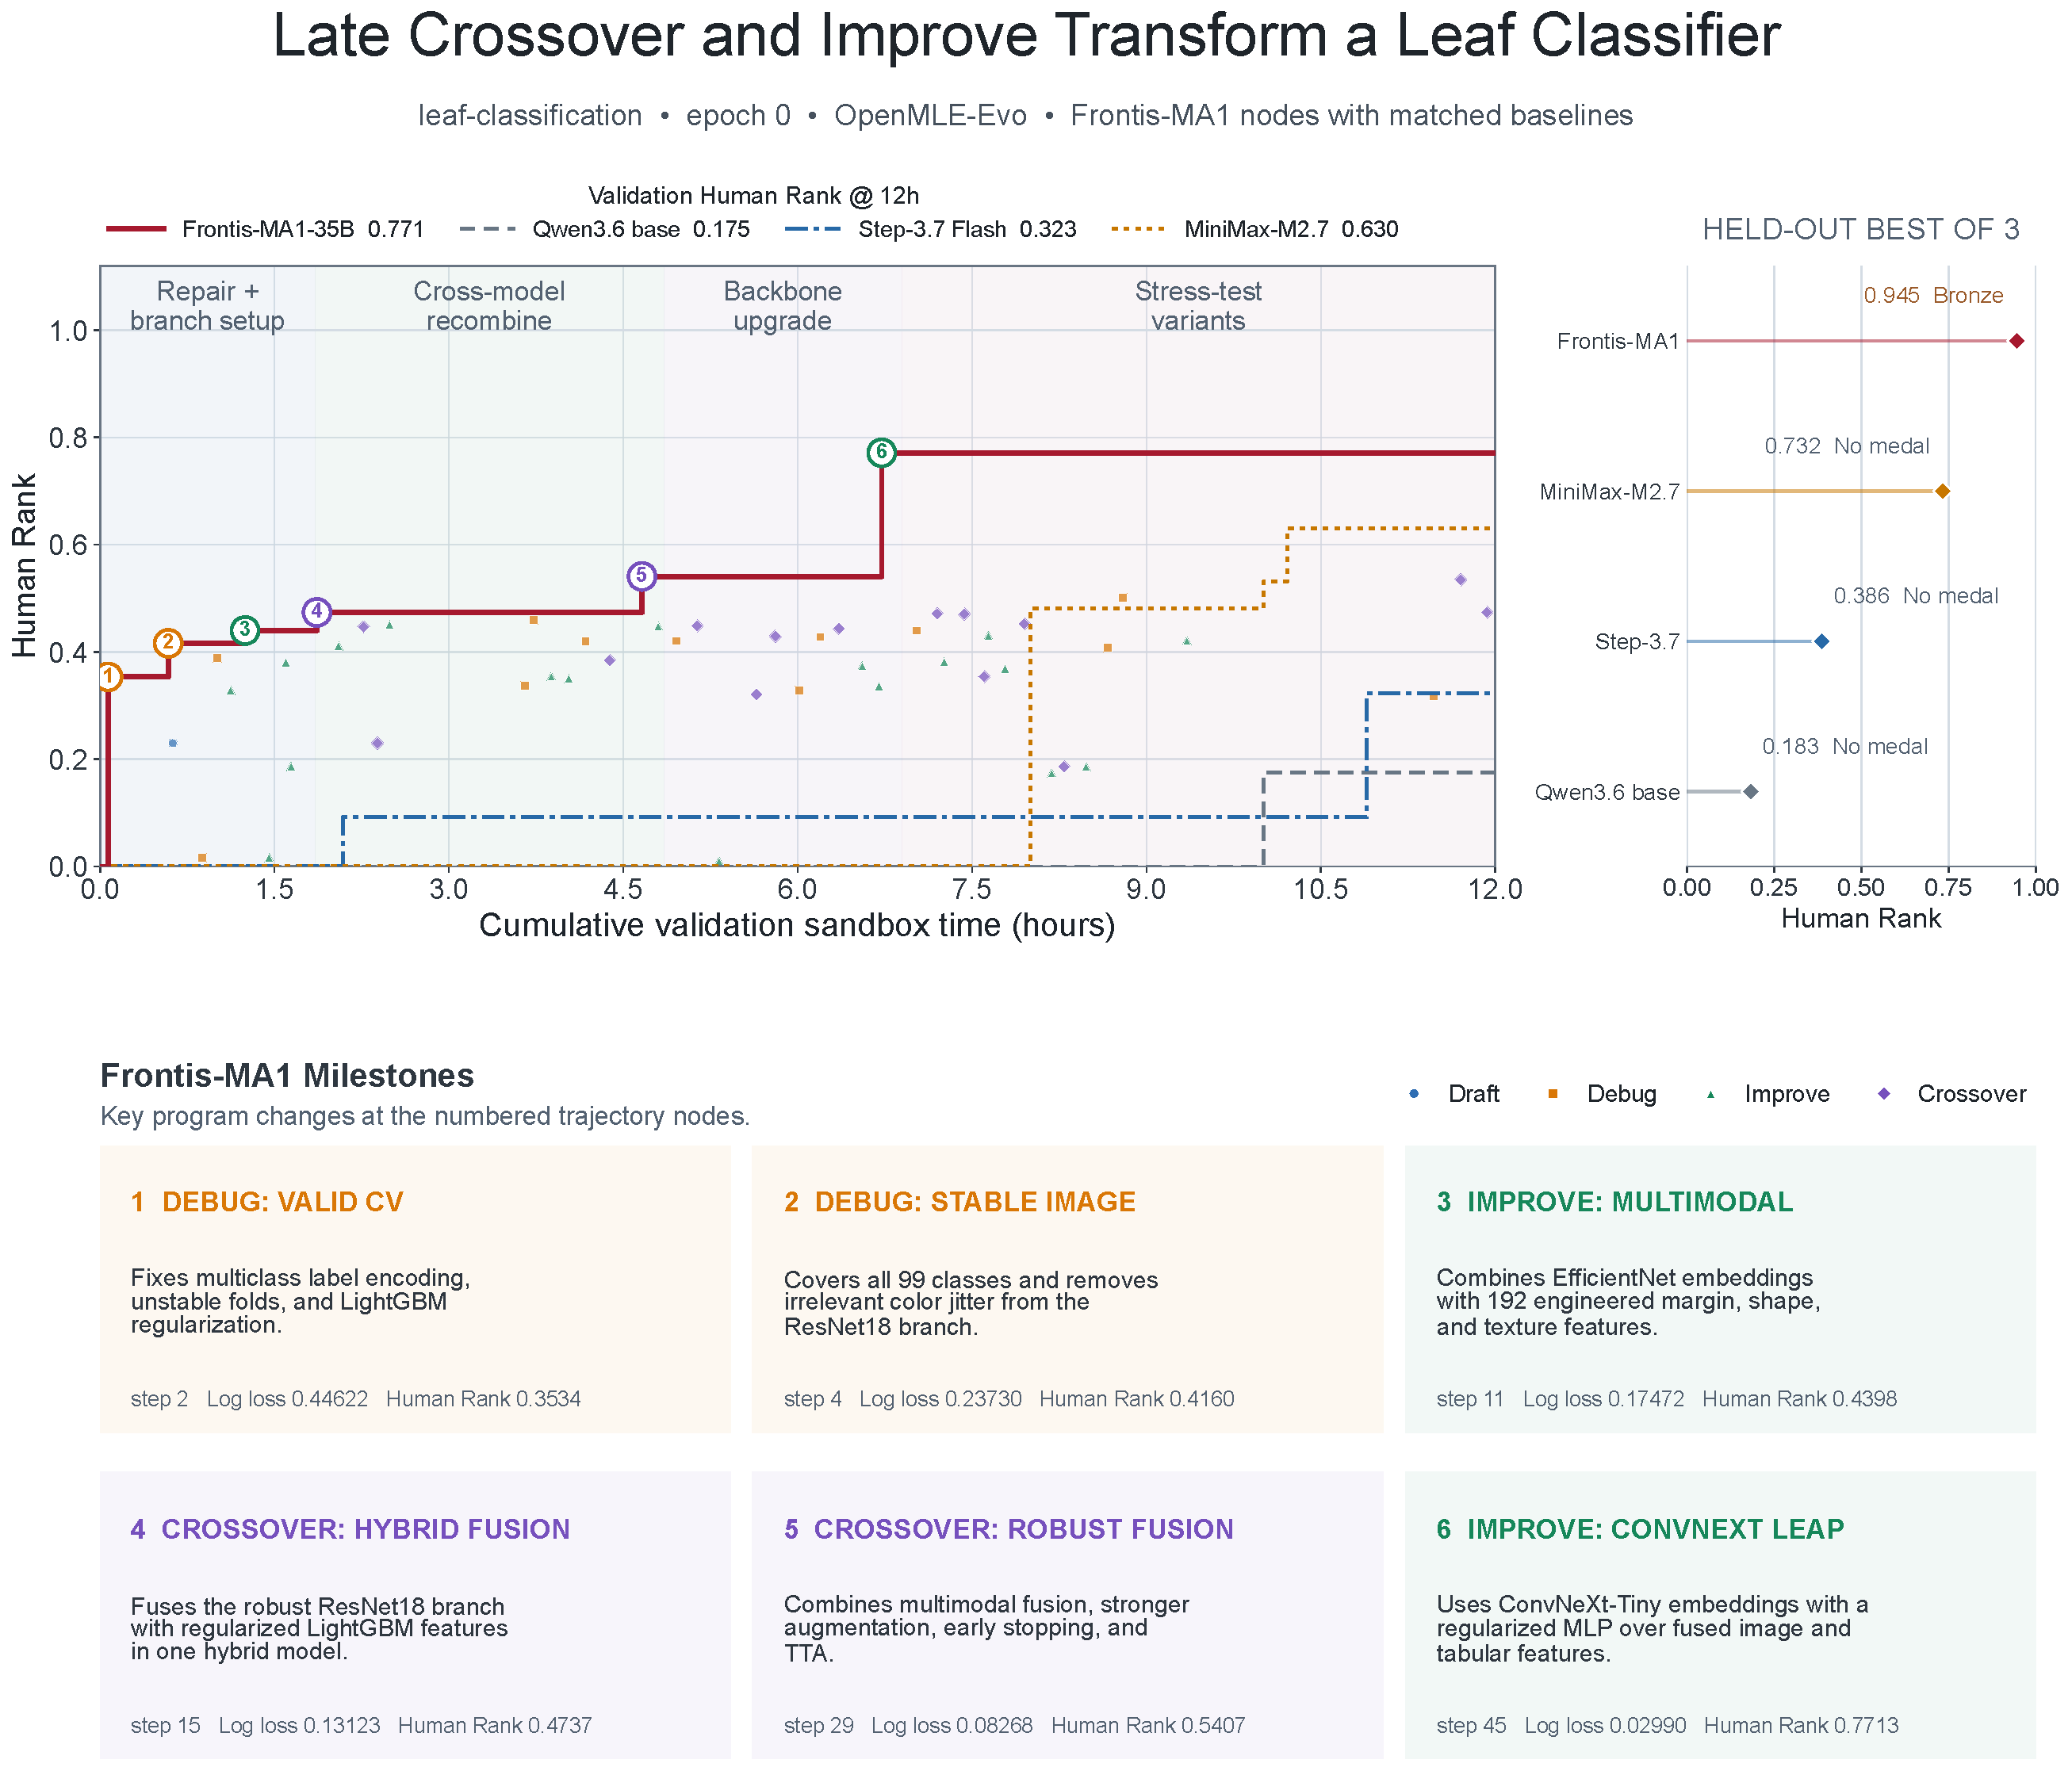
\includegraphics[width=1.0\textwidth]{figures/case_study_leaf_late_operations.pdf}
  \caption{Cross-model search trajectories on \textit{leaf-classification}. The left panel compares best-so-far validation-derived Human Rank over 12 cumulative sandbox hours for the same epoch under the common \openmleevo{} protocol; markers and numbered operation cards expose only the detailed \thirtyfivebmodel{} trajectory. Its two Crossovers establish and strengthen multimodal image--tabular fusion, and a late Improve operation produces the largest jump by upgrading the fused representation to ConvNeXt-Tiny. The separate right panel reports held-out best-of-three final-test Human Rank, where the selected \thirtyfivebmodel{} node obtains Bronze.}
  \label{fig:case-study-leaf-late-ops}
\end{figure}

\subsection{Solution Ceiling}
\label{sec:solution-ceiling}

\begin{takeaway}
Within matched model and search comparisons, the gains are not limited to moving more solutions across the Bronze threshold: stronger systems also produce a larger share of Gold solutions.
\end{takeaway}

Figure~\ref{fig:solution-ceiling-medals} reveals a consistent qualitative shift for the primary 35B model: post-training and \openmleevomax{} do not merely increase medal coverage, but move successful solutions toward Gold.
The companion 30B comparison reproduces the same direction of change, while the fixed-model GLM-5.2 and MiniMax M3 comparisons show that the pattern also extends to search improvements. Together, these results indicate improved solution quality rather than only more Bronze-threshold crossings. Compared with external systems, \thirtyfivebmodel{} with \openmleevomax{} outperforms Claude Opus 4.8 with Claude Code and Gemini 3.5 Flash with Gemini CLI, and matches Kimi K3's Gold rate.

\begin{figure}[!t]
  \centering
  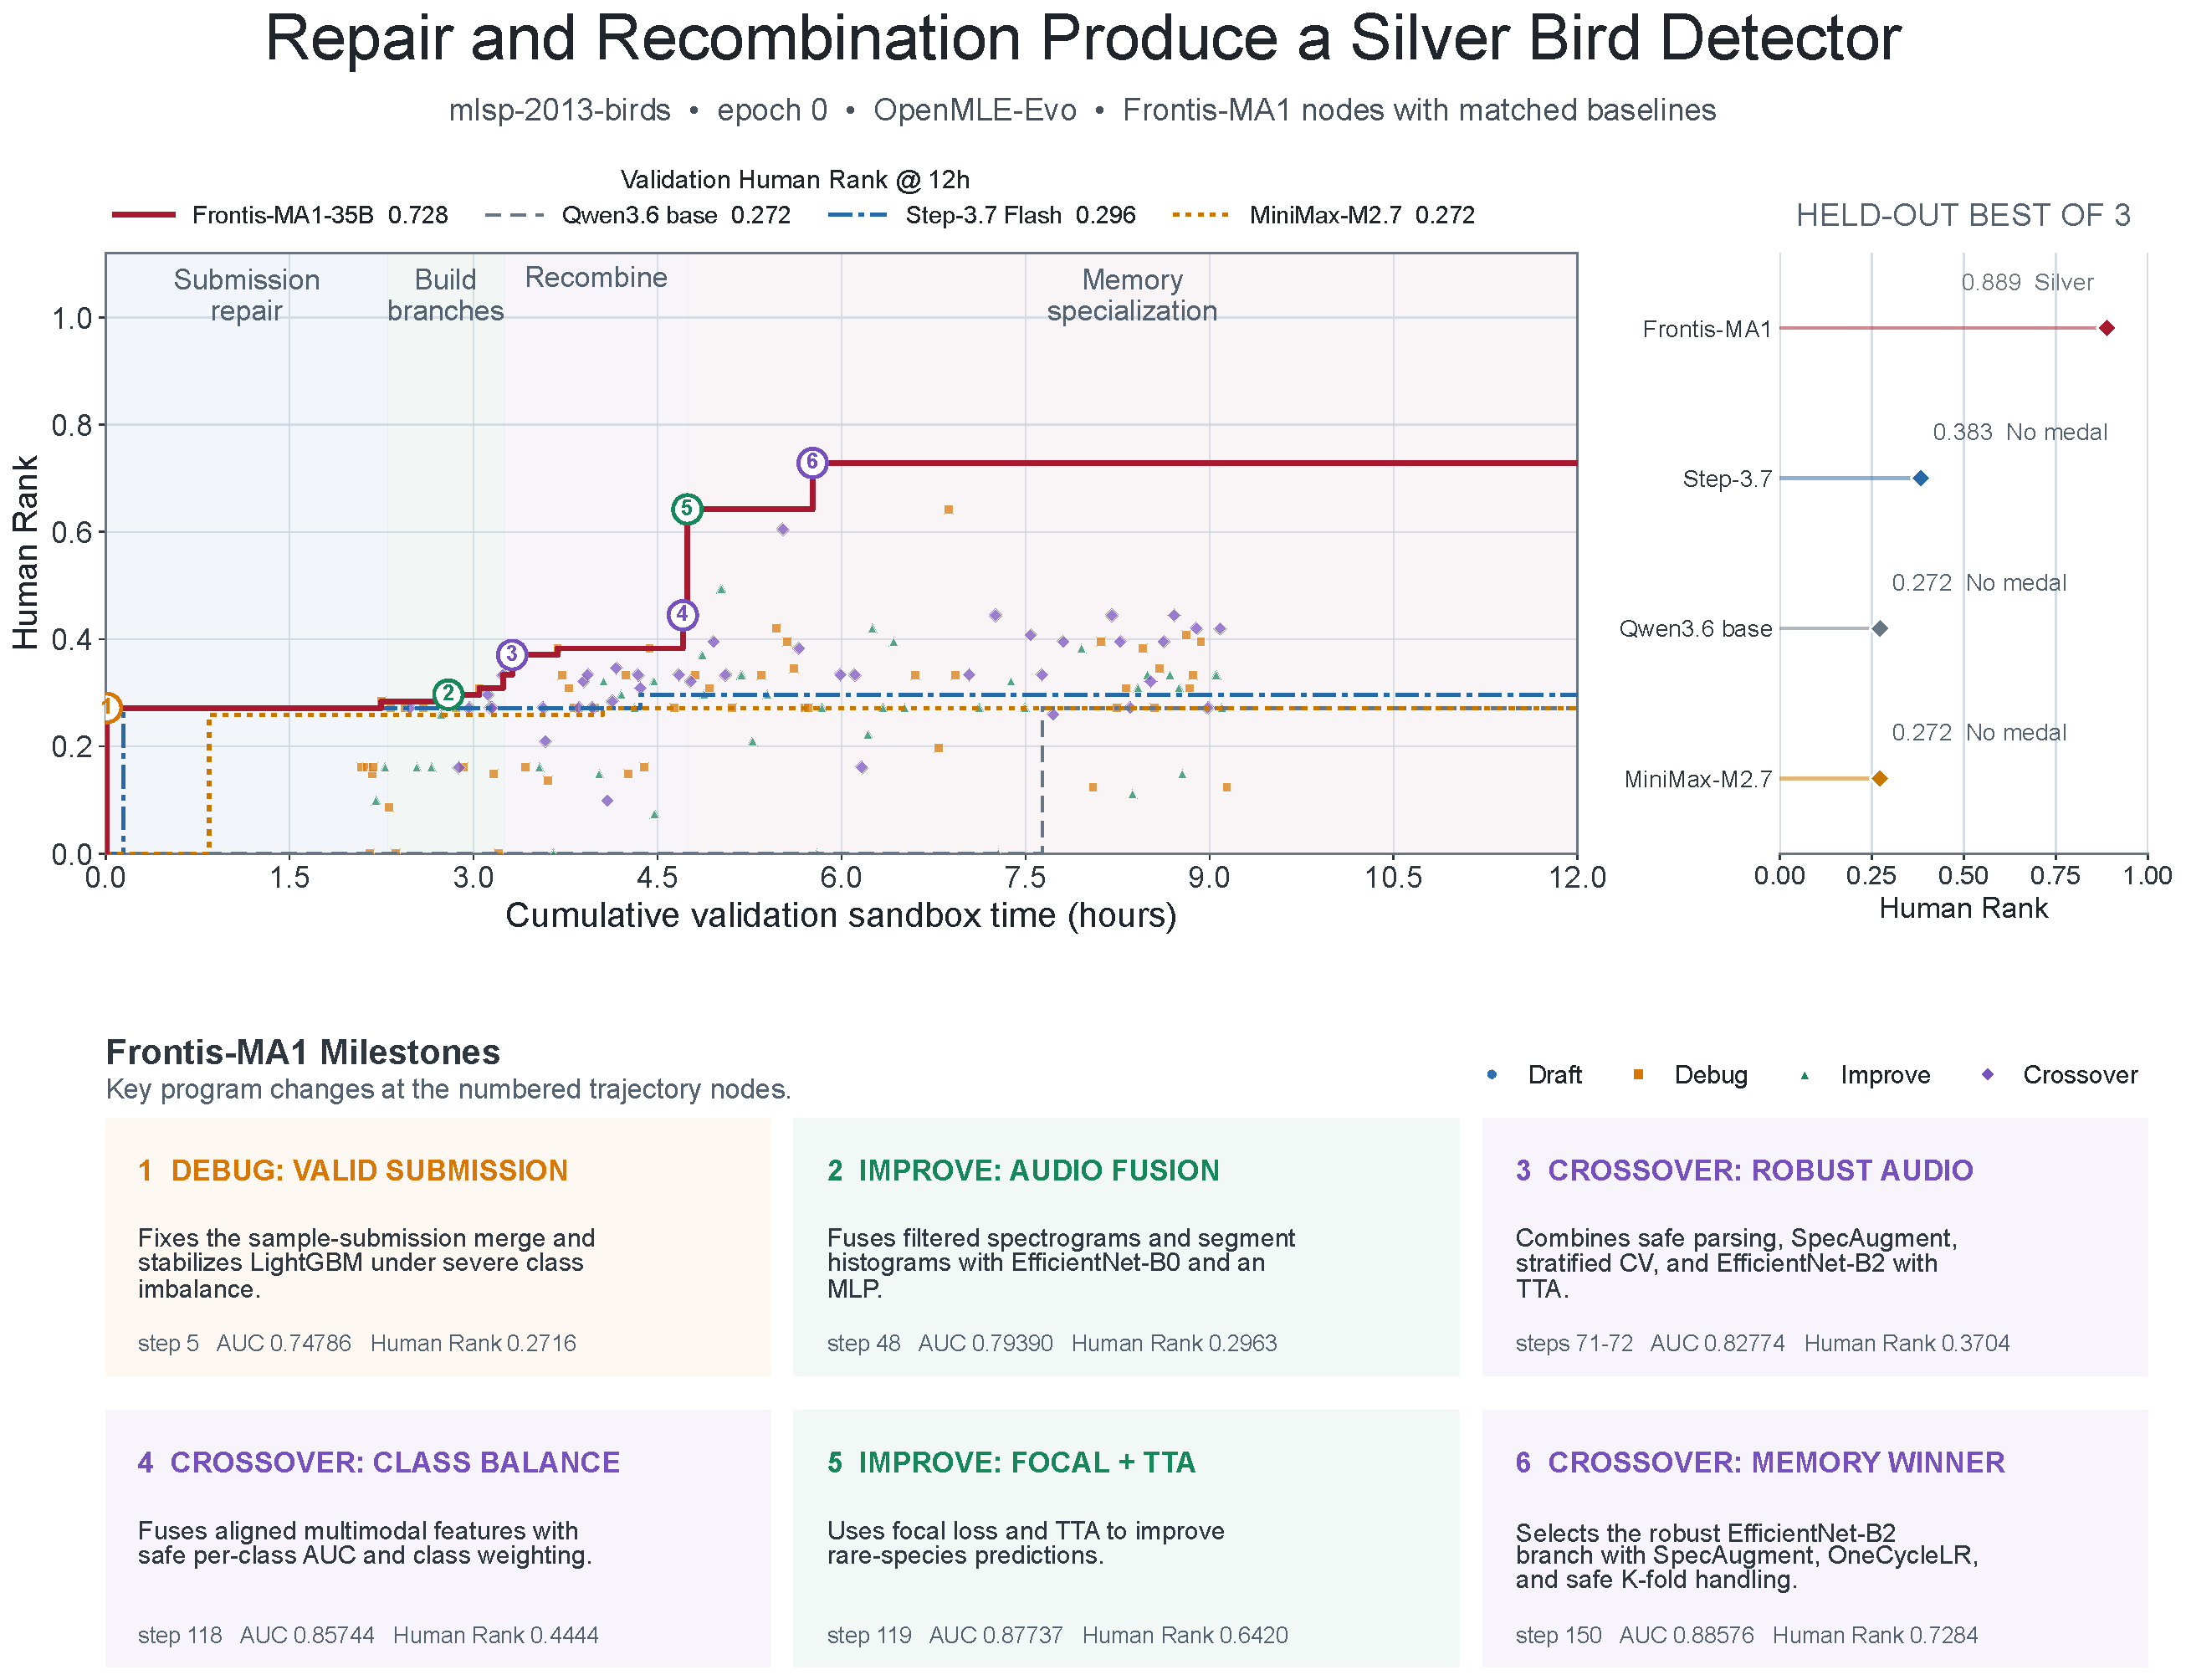
\includegraphics[width=1.0\textwidth]{figures/case_study_mlsp_operation_chain.pdf}
  \caption{Cross-model search trajectories on \textit{mlsp-2013-birds} using the same corrected task prompt. The left panel compares best-so-far validation-derived Human Rank over 12 cumulative sandbox hours under the common \openmleevo{} protocol; markers and numbered operation cards expose only the detailed \thirtyfivebmodel{} trajectory. Early Debug makes the submission executable, while later Improve and Crossover operations build progressively stronger multimodal audio branches. The separate right panel reports held-out best-of-three final-test Human Rank, where the final Memory-guided Crossover obtains Silver.}
  \label{fig:case-study-mlsp-operation-chain}
\end{figure}

\begin{figure}[htbp]
  \centering
  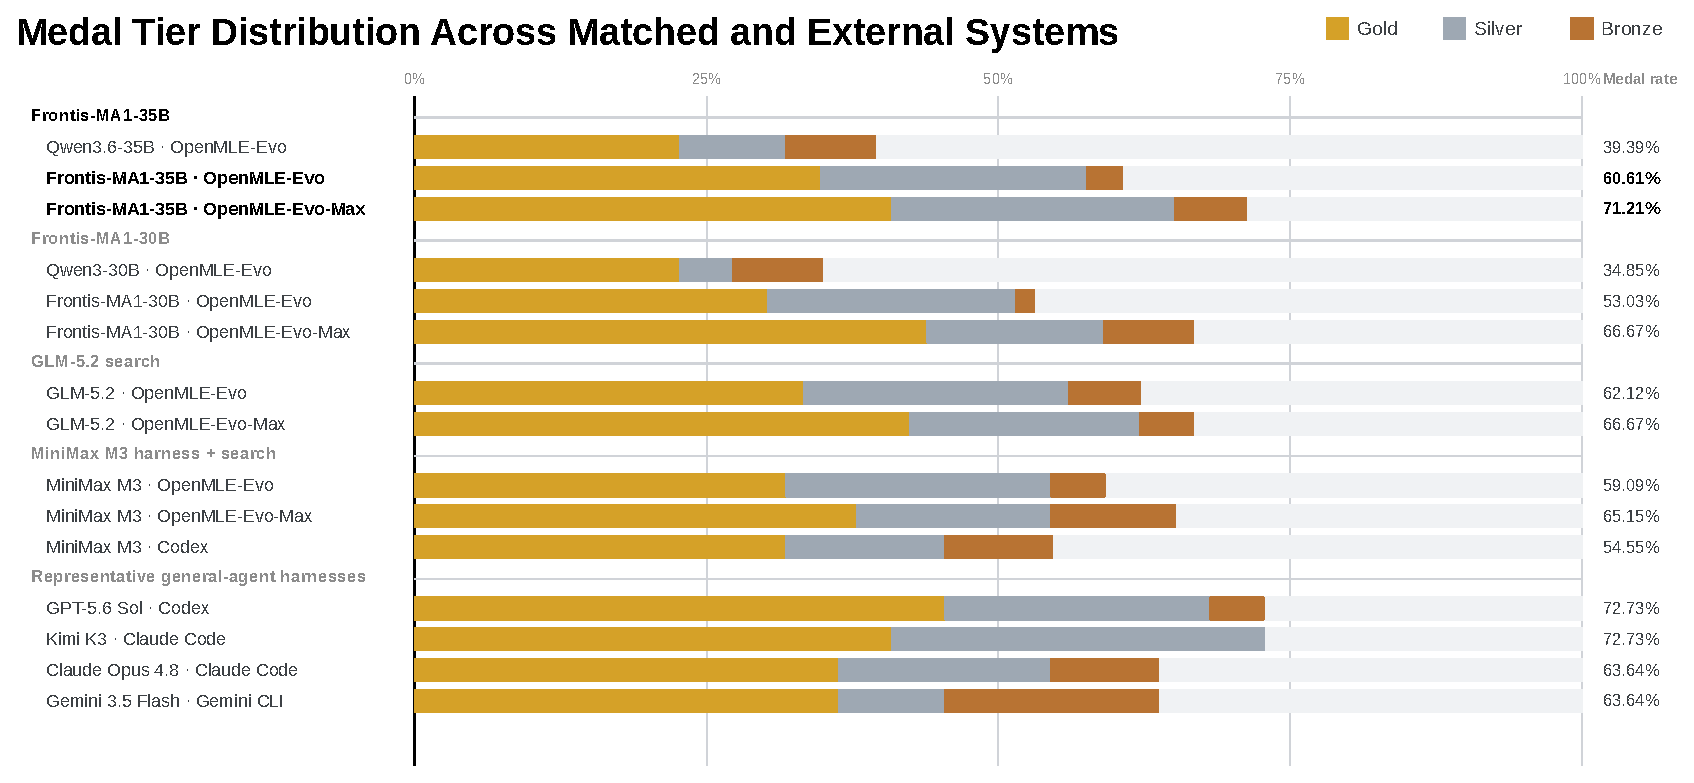
\includegraphics[width=1.0\textwidth]{figures/solution_ceiling_medals.pdf}
  \caption{Gold, Silver, and Bronze decomposition for matched OpenMLE comparisons and representative general-agent harnesses. Bar lengths report the fraction of evaluated outcomes at each medal tier; labels report the final Medal Rate.}
  \label{fig:solution-ceiling-medals}
\end{figure}

\subsection{Search Efficiency and Mechanism}
\label{sec:search-efficiency-mechanism}

\begin{takeaway}
The available trajectory evidence indicates that bounded, operation-conditioned context can improve search productivity while targeted recombination and multi-factor parent selection preserve complementary hypotheses that score-only lineage search may discard.
\end{takeaway}
\paragraph{OpenMLE-Evo versus original AIRA-Evo.}
Figure~\ref{fig:search-efficiency-mechanism} compares complete single-worker trajectories from the same \thirtyfivebmodel{} checkpoint under the same seed and 12-hour task budget, covering 66 task--run evaluations per harness.
\textbf{Lower search cost.}
Panel A shows that \openmleevo{} reduces total model-token consumption from $129.3$M to $75.3$M ($-41.7\%$) and prompt tokens from $83.5$M to $41.5$M ($-50.3\%$), while the number of evaluated nodes falls only from $3430$ to $3004$ ($-12.4\%$).
The much larger reduction in tokens than in nodes indicates that the saving comes primarily from making each expansion cheaper, not merely from terminating the search earlier or evaluating far fewer candidates.
\textbf{Higher search yield.}
Panel B counts a new-best validation update whenever a node strictly improves the task--run's best selection reward after its first finite result.
Although it evaluates fewer nodes, \openmleevo{} records 246 such updates rather than 229, raising new-best updates per million total model tokens from $1.77$ to $3.27$ ($+84.3\%$).
The fraction of \textsc{Improve} operations that establish a new best likewise rises from $44/931$ ($4.73\%$) to $72/769$ ($9.36\%$), showing that refinement calls are more likely to produce useful progress.
\textbf{Bounded operation context.}
Panel C connects this improved yield to the intended context mechanism.
For \textsc{Improve}, the mean serialized user-prompt length falls from $102.8$K to $35.7$K Unicode characters ($-65.3\%$), and its 99th percentile falls from $389.0$K to $54.3$K ($-86.1\%$).
For \textsc{Crossover}, the corresponding mean falls from $140.4$K to $55.3$K ($-60.6\%$), while the 99th percentile falls from $419.2$K to $78.4$K ($-81.3\%$).
The compression is especially strong in the tail, consistent with structured operation-conditioned memory preventing long histories from being repeatedly serialized into every request.
Together, the panels show that \openmleevo{} improves the productivity of each refinement.
We characterize search efficiency using token usage, context length, and validation-trajectory productivity.

\begin{figure*}[htbp]
  \centering
  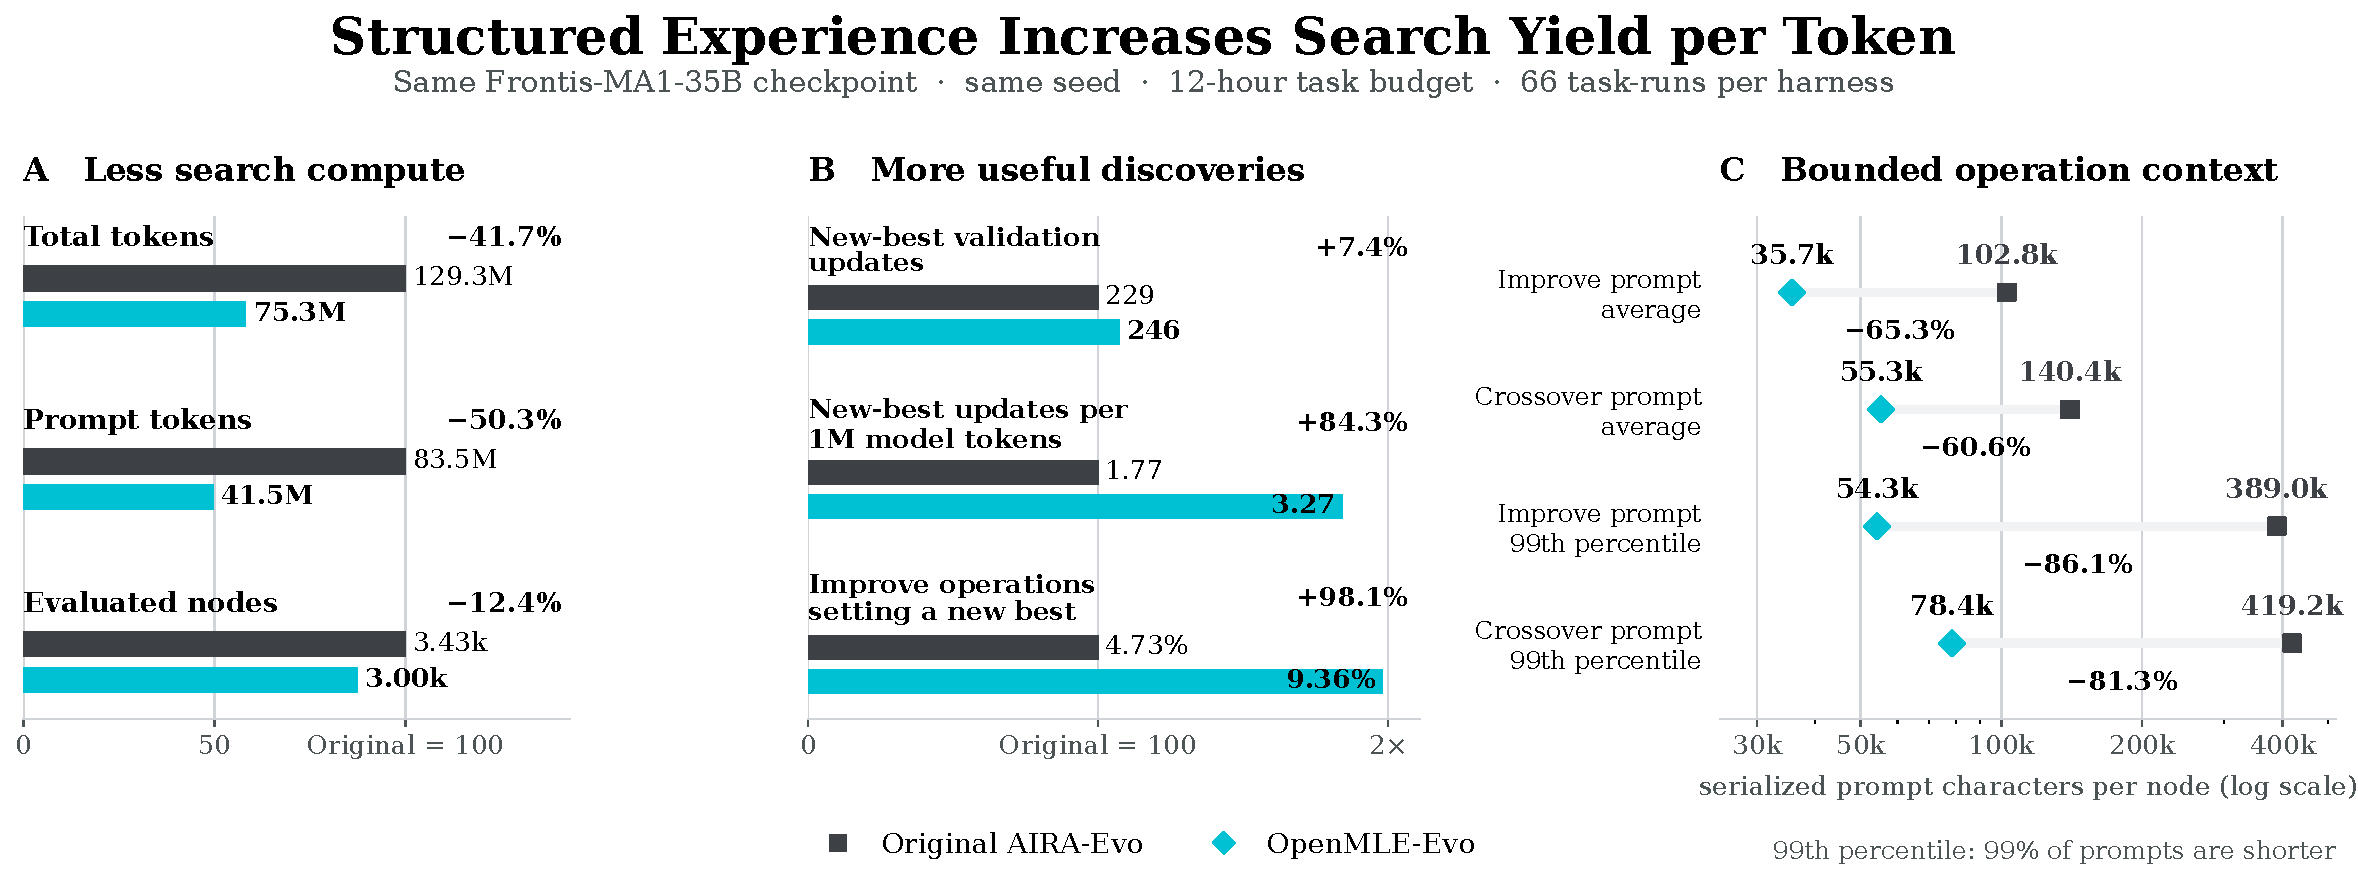
\includegraphics[width=0.99\textwidth]{figures/search_efficiency_mechanism.pdf}
  \caption{Search efficiency and context-length comparison between original AIRA-Evo (gray) and \openmleevo{} (cyan) over 66 matched task--runs. Panel A normalizes each resource metric to original AIRA-Evo${}=100$ and annotates the absolute totals. Panel B reports validation-trajectory productivity. A ``new-best validation update'' is a strict increase in selection reward after a task--run's first finite score; the per-million-token denominator includes both prompt and completion tokens, and the \textsc{Improve} rate is the fraction of \textsc{Improve} operations that set a new best. Panel C reports serialized user-prompt length in Unicode characters on a logarithmic axis; the 99th percentile is the length below which 99\% of prompts fall.}
  \label{fig:search-efficiency-mechanism}
\end{figure*}

\textbf{Targeted Crossover escapes a single-branch Debug loop.}
Figure~\ref{fig:case-study-nomad-targeted-crossover} contrasts two grounded \textit{nomad2018-predict-transparent-conductors} traces. Original AIRA-Evo follows a single lineage after its Draft fails: seven successive \textsc{Debug} attempts inherit an expanding full history, and the final repair reaches validation RMSE $0.06633$ and held-out RMSE $0.06096$. The \openmleevo{} trace instead constructs a targeted \textsc{Crossover} at step 81 from complementary evidence. One parent contributes atomic properties, dynamic covalent edges, and unit-cell volume (validation RMSE $0.06309$); the other contributes a robust parser for irregular \texttt{.xyz} geometries (validation RMSE $0.06573$). Horizontal Memory also marks an RDF-cache \texttt{TypeError} and a $3328 \times 94$ feature mismatch as negative evidence, thereby avoiding their silent serialization into the child context. The resulting program combines the physics-informed GNN with the robust parser, density descriptors, and cosine scheduling, reaching validation RMSE $0.06087$ and held-out RMSE $0.05410$, respectively $8.2\%$ and $11.3\%$ below the original trace. The comparison illustrates the intended mechanism: operation-conditioned Memory converts distinct branch strengths and known failures into a bounded recombination request instead of repeatedly repairing one lineage.

\begin{figure*}[htbp]
  \centering
  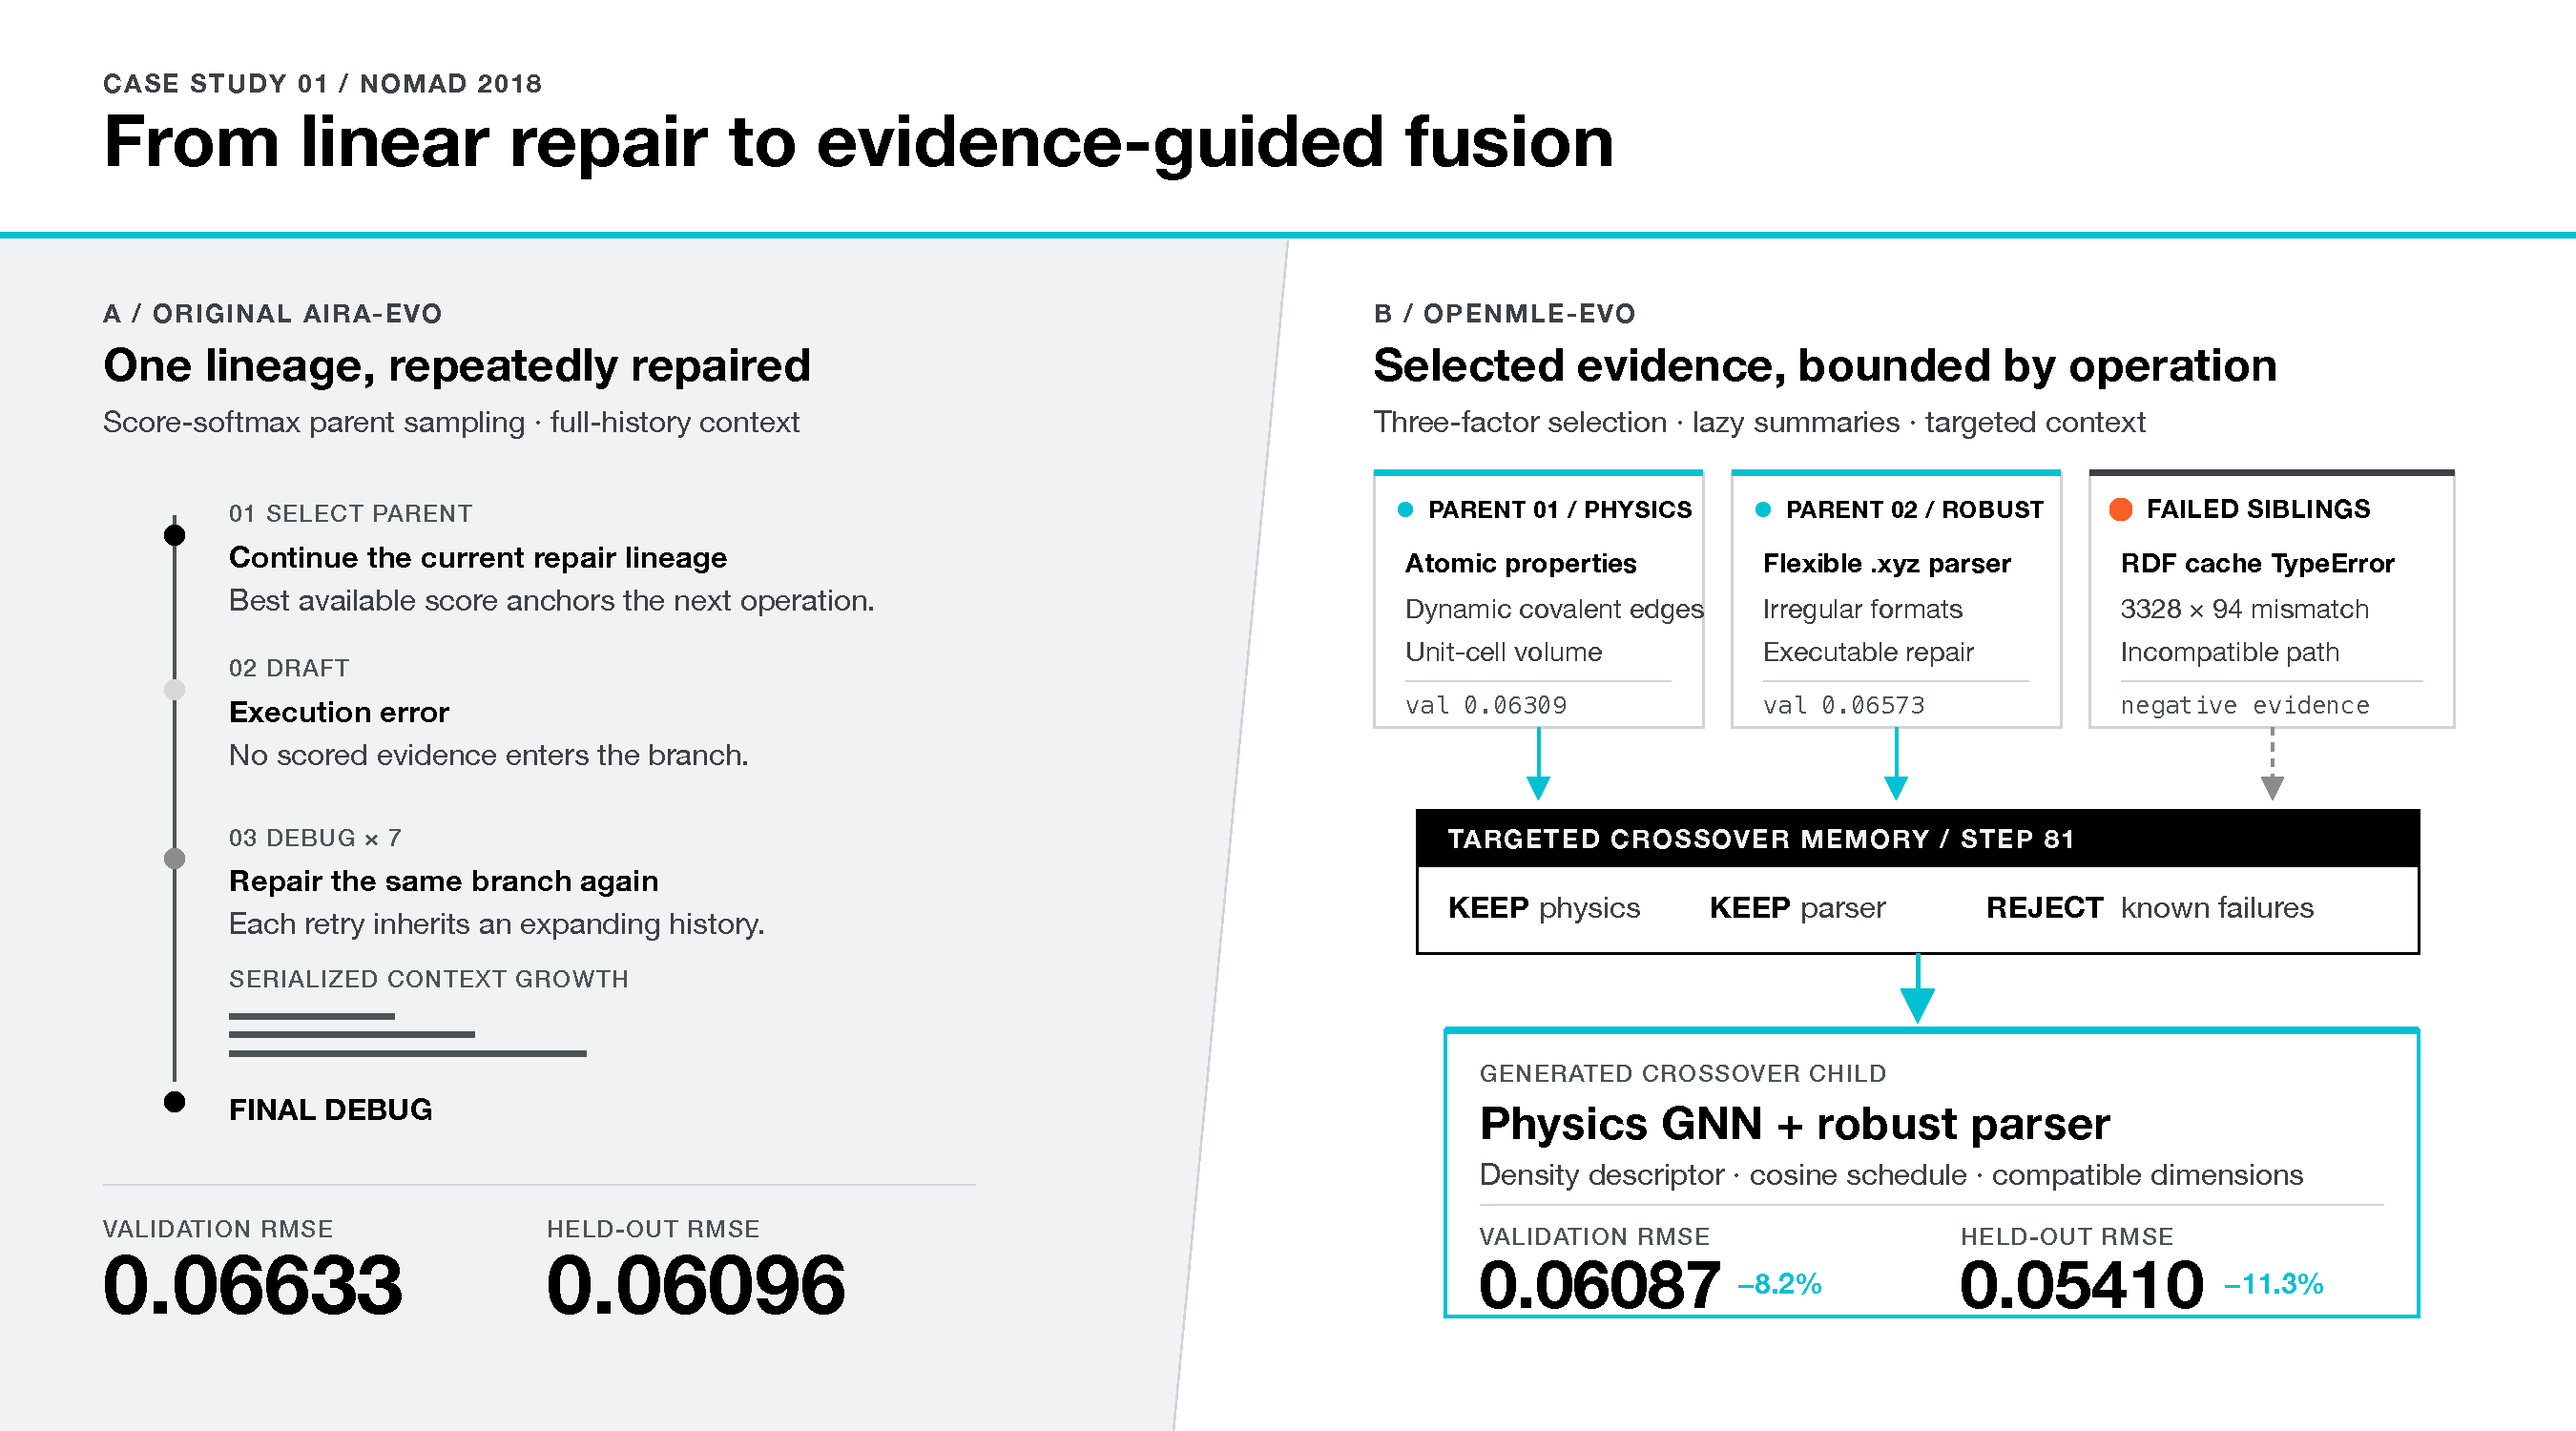
\includegraphics[width=0.98\textwidth]{figures/case_study_nomad_targeted_crossover1.pdf}
  \caption{Single-branch repair versus targeted Crossover on \textit{nomad2018-predict-transparent-conductors}. Original AIRA-Evo repeatedly debugs one lineage using full-history context. \openmleevo{} selects complementary physics and parsing parents, excludes failures observed in nearby siblings, and forms an operation-bounded Crossover child. Lower RMSE is better.}
  \label{fig:case-study-nomad-targeted-crossover}
\end{figure*}

\textbf{Three-factor selection preserves a complementary parent.}
Figure~\ref{fig:case-study-right-whale-three-factor} shows why selecting parents by current score alone can discard useful structure on \textit{the-icml-2013-whale-challenge-right-whale-redux}. In the original AIRA-Evo trace, two independently repaired branches reach validation AUCs $0.94656$ and $0.85546$; score-only selection keeps the stronger branch, producing held-out AUC $0.94852$. The \openmleevo{} step-10 candidate pool exposes a subtler choice. Parent A is the score leader at AUC $0.99187$ and provides a deeper ResNet-SE pipeline with 64-Mel features, AMP, and test-time augmentation. Parent B scores slightly lower at $0.98773$ and ranks only sixth by score, but ranks first by gain after improving $0.00568$ over its own parent; it retains a promising Log-Mel representation with Delta and Delta-Delta temporal channels. With Score/Gain/Novelty weights $1.0/0.6/0.3$, Parent B moves to the top utility rank, and its selection probability within the same ten-parent pool increases from $10.47\%$ under score-only softmax to $17.09\%$, a $63.2\%$ relative increase. Parent B is then selected for an \textsc{Improve} operation, whose child reaches validation AUC $0.99203$ and held-out AUC $0.99386$. This within-pool probability recomputation directly exposes the selector's effect: the additional factors do not force a lower-scoring branch to win, but keep a high-gain, structurally distinct branch actionable long enough to be selected and refined. Because the full framework also changes targeted Memory, the end-to-end difference from original AIRA-Evo should not be attributed to the three weights alone.

\begin{figure*}[htbp]
  \centering
  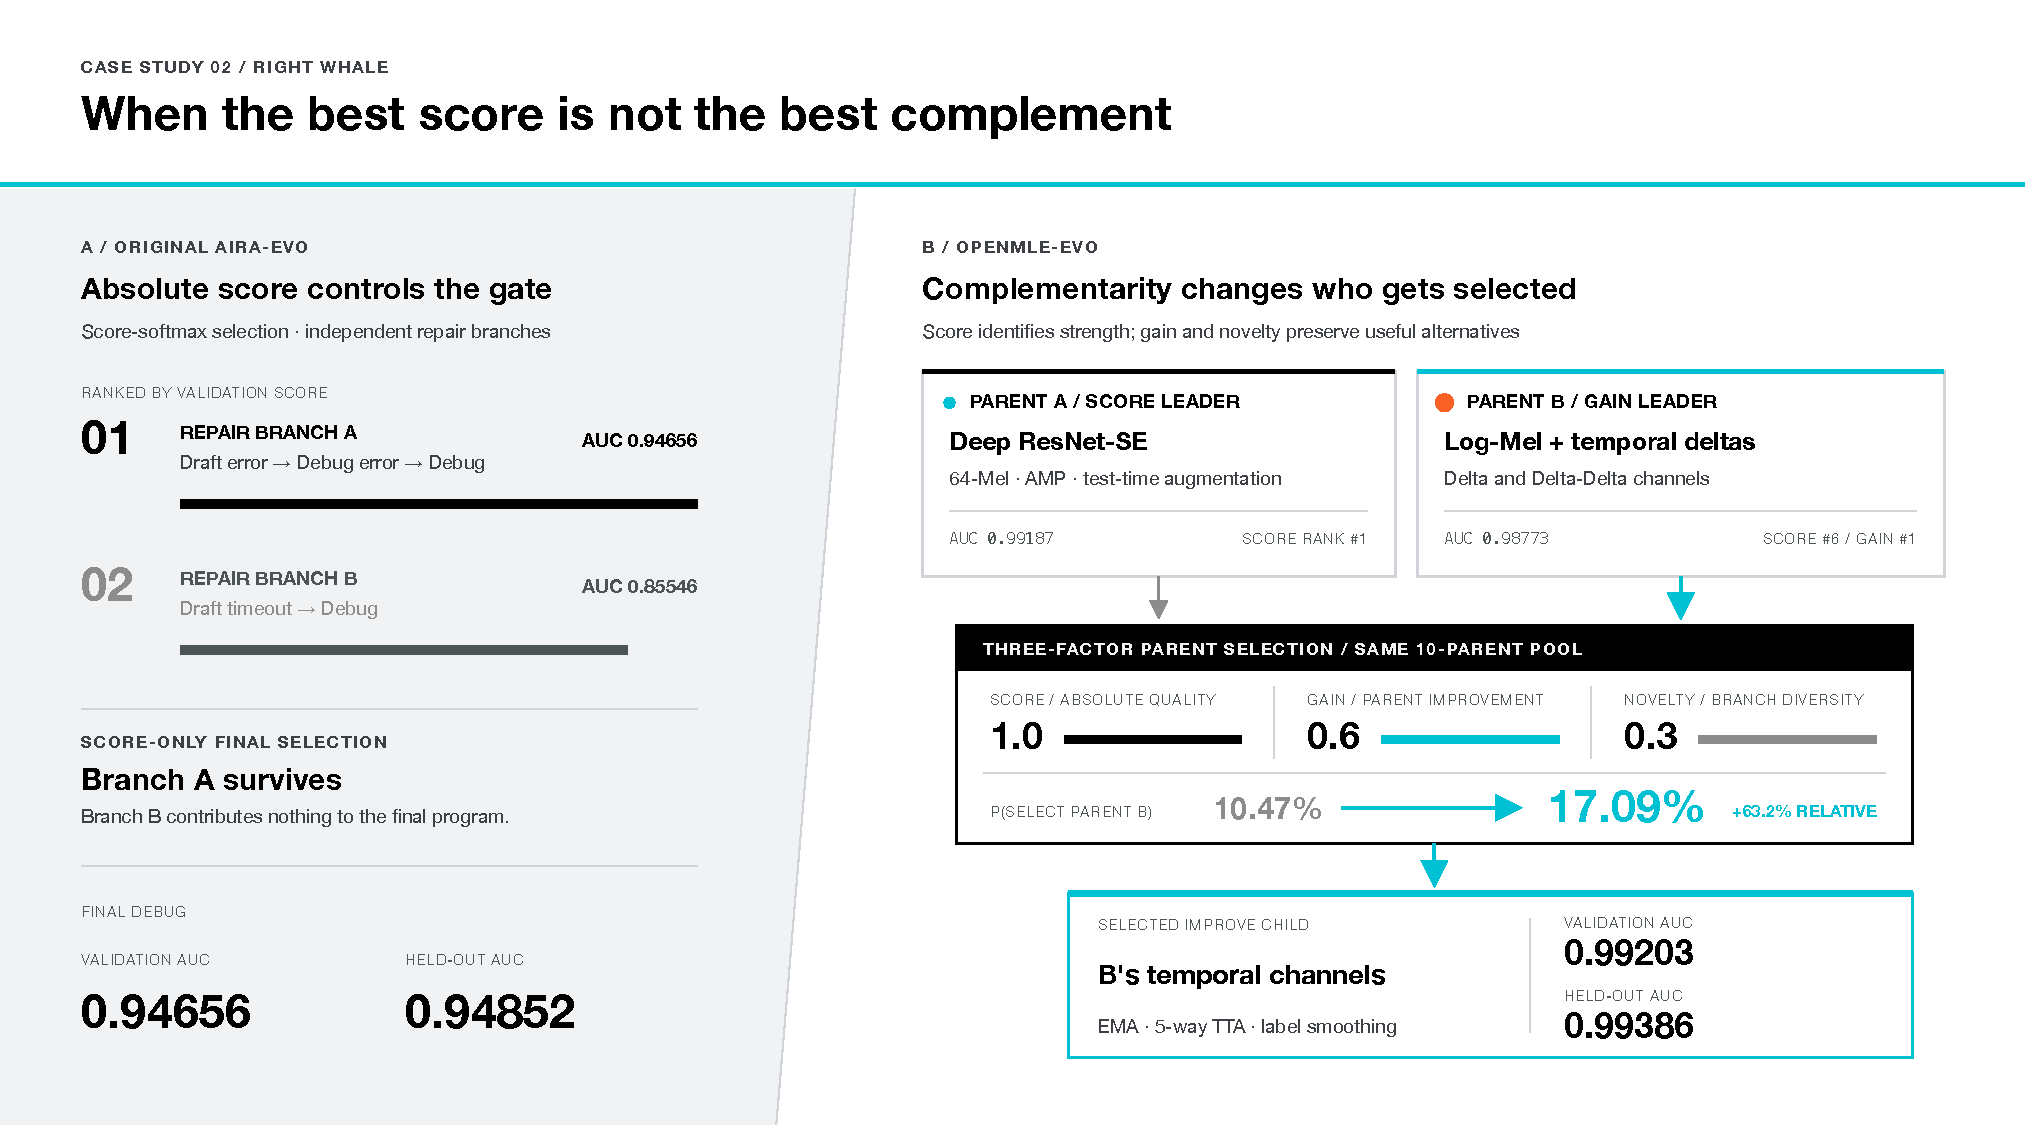
\includegraphics[width=0.98\textwidth]{figures/case_study_right_whale_three_factor_selection.pdf}
  \caption{Score-only versus three-factor parent selection on right-whale detection. Parent A leads in current validation AUC, whereas Parent B ranks sixth by score but first by gain and retains promising temporal channels. Score/Gain/Novelty weighting raises Parent B's selection probability from $10.47\%$ to $17.09\%$ over the same ten-parent pool, enabling an Improve child derived from Parent B. Higher AUC is better.}
  \label{fig:case-study-right-whale-three-factor}
\end{figure*}


\subsection{Meta-Ability and Transfer}
\label{sec:meta-ability-transfer}

\begin{takeaway}
Modality-stratified MLE-Bench results show broad gains across data types, and controlled NatureBench Lite results provide initial evidence of transfer beyond competition-style MLE; small modality groups and the ten-task transfer set limit the breadth of both conclusions.
\end{takeaway}
\paragraph{Cross-modality meta-ability on MLE-Bench.}
Before testing out-of-benchmark transfer, we ask whether the learned improvement capability is tied to a narrow input modality.
We partition the 22 MLE-Bench Lite tasks into five mutually exclusive groups: image, text, tabular/structured, audio, and multimodal.
Relative to Qwen3.6-35B-A3B under the same \openmleevo{} harness, \thirtyfivebmodel{} raises mean Human Rank in all five groups and never lowers group-level Medal Rate (Figure~\ref{fig:mle-modality-stratified}).
The 14 additional medals are distributed across every group (image/text/tabular/audio/multimodal: $+2/+4/+1/+4/+3$), so the aggregate gain is not explained by one modality alone.


\paragraph{Generalization to NatureBench.}
\label{sec:naturebench}

NatureBench evaluates whether coding agents can recover or improve upon published scientific results~\citep{wang2026naturebench}.
Its full benchmark contains 90 containerized tasks distilled from peer-reviewed Nature-family papers across six scientific domains.
Each task hides the test ground truth and paper method behind a host-side evaluator, and compares heterogeneous scientific metrics through the direction-normalized relative gap
\begin{equation}
g = \mathrm{dir}\,\frac{m-m_{\mathrm{SOTA}}}{|m_{\mathrm{SOTA}}|},
\label{eq:naturebench-gap}
\end{equation}
where $m$ is the submitted result and $\mathrm{dir}\in\{-1,+1\}$ accounts for whether the task metric is minimized or maximized.
We report \emph{Match-SOTA} (All M), the fraction of tasks with $g\geq 0$, and \emph{Surpass-SOTA} (All S), the stricter fraction with $g>0.1$.

\begin{figure}[htbp]
  \centering
  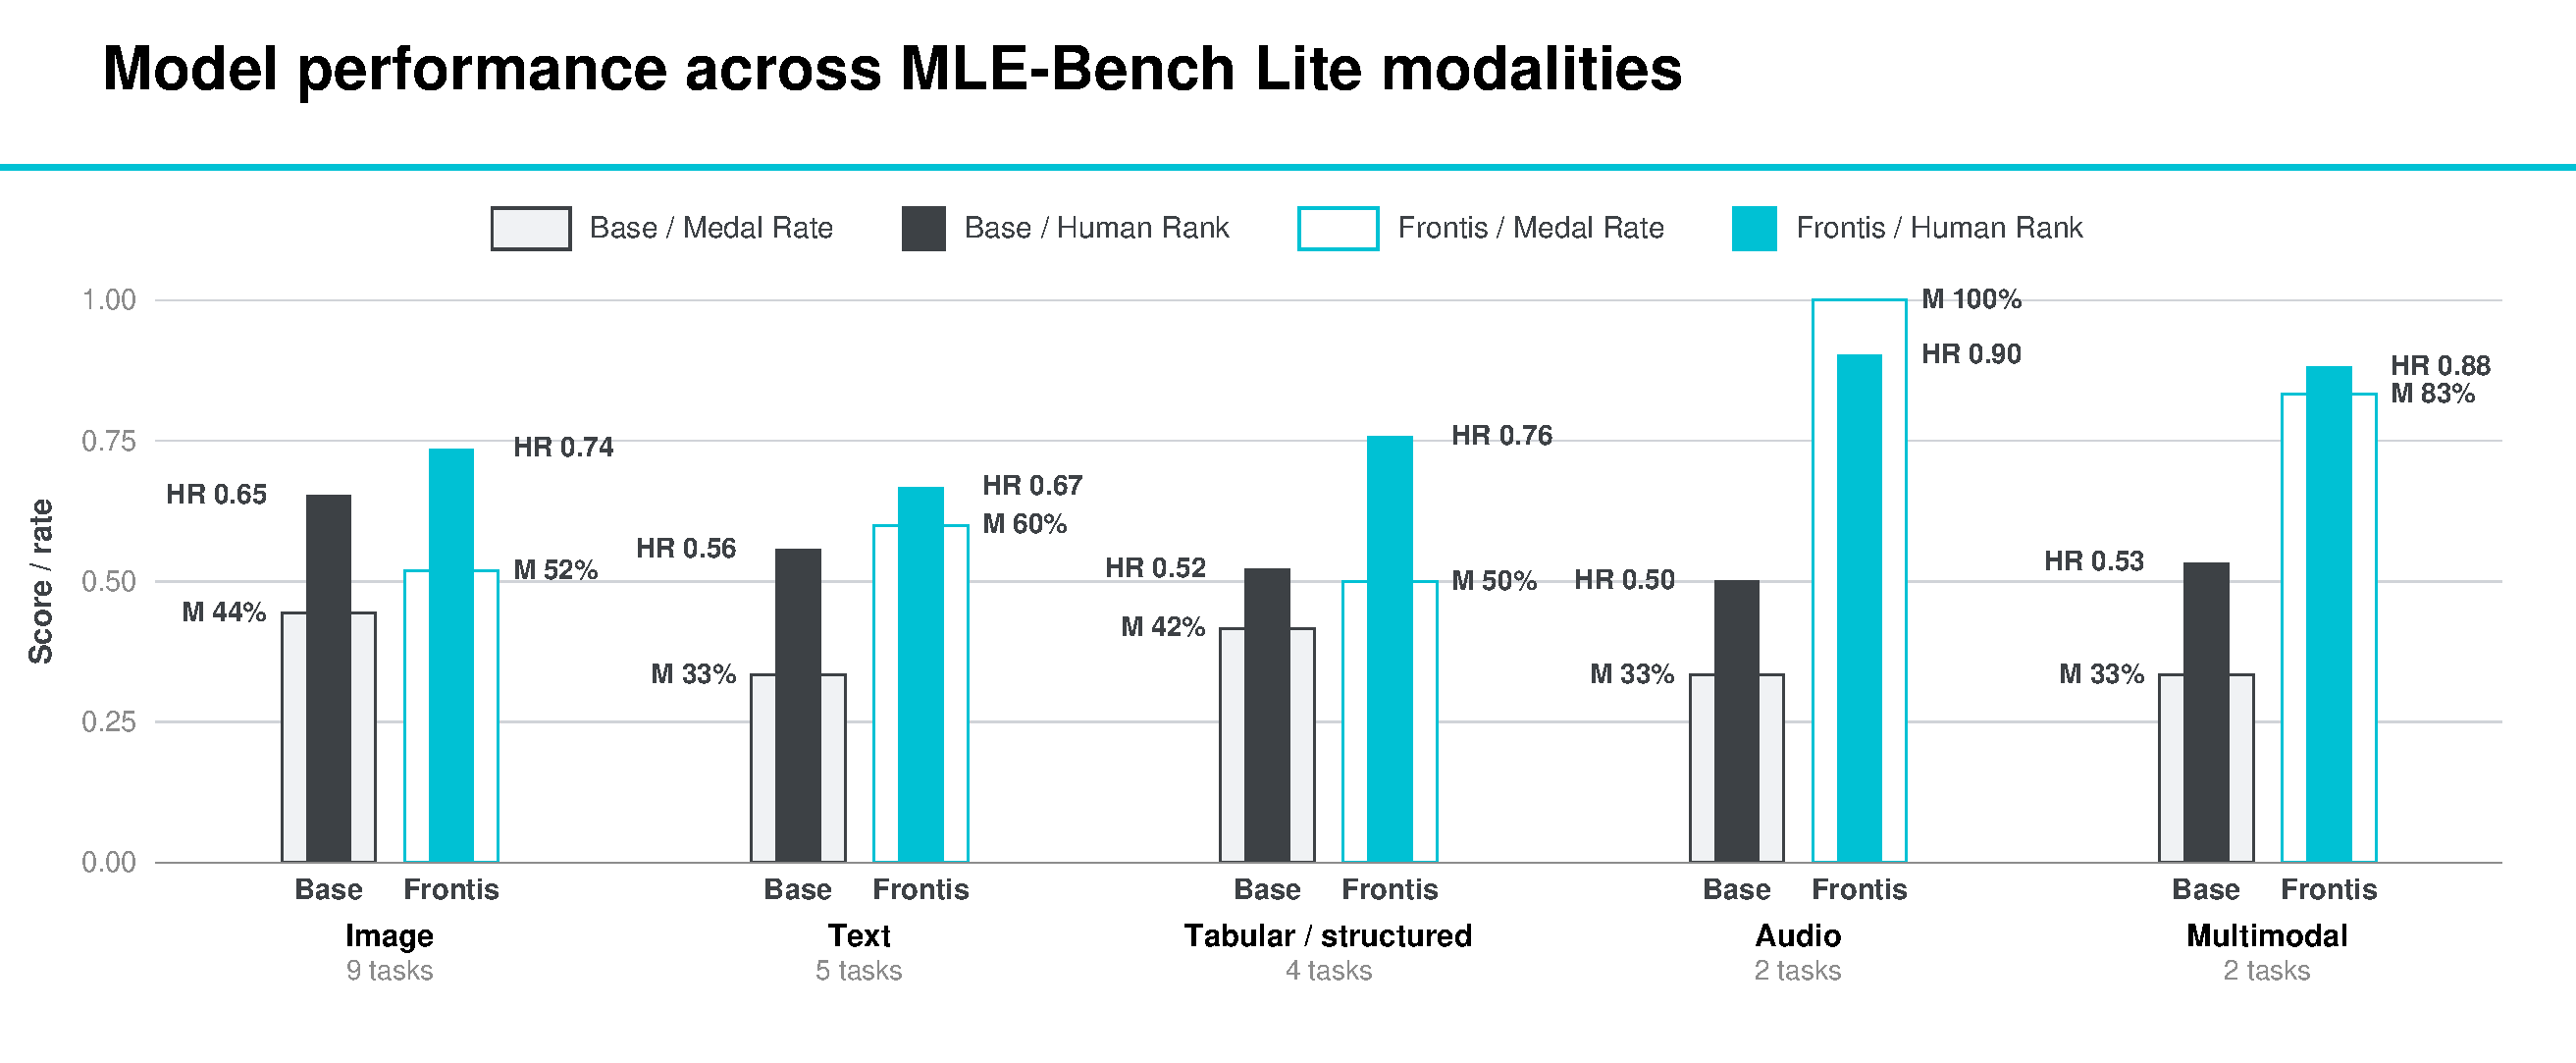
\includegraphics[width=\textwidth]{figures/model_performance_across_mle_bench_lite_modalities.pdf}
  \caption{Modality-stratified results on the MLE-Bench Lite subset. Base denotes Qwen3.6-35B-A3B and Frontis denotes \thirtyfivebmodel{}, both evaluated with \openmleevo{}. Wide outlined bars show Medal Rate, and narrow filled bars show mean Human Rank; both use all three task--epoch outcomes per task, with invalid final submissions assigned zero Human Rank. }
  \label{fig:mle-modality-stratified}
\end{figure}

For a tractable but heterogeneous transfer study, we use NatureBench Lite, a fixed 10-task subset spanning all six domains, six represented input-modality families, and four ML task types; Appendix~\ref{app:naturebench-lite} lists the tasks.
We retain the NatureBench task containers, hidden evaluator, validity rules, web-search-disabled setting, and four-hour search budget per task.
The \openmleevo{} NatureBench adapter changes the task interface, resource scheduling, and feedback plumbing needed to run the same evolutionary program operators against NatureBench's evaluator; it does not expose hidden labels or the paper solution.
Table~\ref{tab:naturebench-lite-results} reports the reference agent results and our controlled model--harness comparisons.


The transfer results expose contributions from both the post-trained model and the adapted search framework.
Holding the NatureBench adapter fixed, \thirtyfivebmodel{} improves over its Qwen3.6-35B-A3B base by 10 percentage points in All S ($3/10$ versus $2/10$) and 20 points in All M ($7/10$ versus $5/10$).
Holding the base model fixed, the \openmleevo{} NatureBench adapter improves over original AIRA-Evo by 10 points in All S ($2/10$ versus $1/10$) and 30 points in All M ($5/10$ versus $2/10$).
Consequently, the combined \thirtyfivebmodel{} system matches the $3/10$ All S and $7/10$ All M attained by GPT-5.4, GLM-5.1, and MiniMax-M3 on this subset, and exceeds the reported DeepSeek-V4-Pro, Claude Opus 4.6, and MiniMax-M2.7 configurations.
This provides evidence that execution-grounded post-training transfers beyond competition-style MLE and that the adapted long-horizon search can convert more of that capability into paper-relative scientific progress.

\begin{table}[H]
\centering
\caption{Results on NatureBench (NB) Lite. S and M denote Surpass-SOTA ($g>0.1$) and Match-SOTA ($g\geq 0$), respectively. Public reference agents use Codex for GPT models, Gemini CLI for Gemini 3.5 Flash, and Claude Code for all other models. Bold indicates the best result.}
\label{tab:naturebench-lite-results}
\vspace{0.4em}
\scriptsize
\setlength{\tabcolsep}{3.5pt}
\renewcommand{\arraystretch}{1.06}
\resizebox{\linewidth}{!}{%
\begin{tabular}{@{}cllcc@{}}
\toprule
Rank & Model & Agent harness & All S $\uparrow$ & All M $\uparrow$ \\
\midrule
\multicolumn{5}{@{}l}{\textit{NatureBench Lite reference agents}} \\
1  & Claude Opus 4.7    & Claude Code & \textbf{70.0\% (7/10)} & \textbf{100.0\% (10/10)} \\
2  & GLM-5.2             & Claude Code & \textbf{70.0\% (7/10)} & \textbf{100.0\% (10/10)} \\
3  & Gemini 3.5 Flash    & Gemini CLI  & 60.0\% (6/10) & 80.0\% (8/10) \\
4  & GPT-5.5             & Codex       & 40.0\% (4/10) & \textbf{100.0\% (10/10)} \\
5  & Qwen 3.7 Max        & Claude Code & 40.0\% (4/10) & 60.0\% (6/10) \\
6  & Kimi K2.6           & Claude Code & 30.0\% (3/10) & 90.0\% (9/10) \\
7  & GPT-5.4             & Codex       & 30.0\% (3/10) & 70.0\% (7/10) \\
8  & GLM-5.1             & Claude Code & 30.0\% (3/10) & 70.0\% (7/10) \\
9  & MiniMax-M3          & Claude Code & 30.0\% (3/10) & 70.0\% (7/10) \\
10 & DeepSeek-V4-Pro     & Claude Code & 20.0\% (2/10) & 60.0\% (6/10) \\
11 & Claude Opus 4.6     & Claude Code & 20.0\% (2/10) & 50.0\% (5/10) \\
12 & MiniMax-M2.7        & Claude Code & 0.0\% (0/10)  & 30.0\% (3/10) \\
\midrule
\multicolumn{5}{@{}l}{\textit{OpenMLE controlled comparisons}} \\
-- & \thirtyfivebmodel{} & \openmleevo{} NB adapter & \textbf{30.0\% (3/10)} & \textbf{70.0\% (7/10)} \\
-- & Qwen3.6-35B-A3B & \openmleevo{} NB adapter & 20.0\% (2/10) & 50.0\% (5/10) \\
-- & Qwen3.6-35B-A3B & Original AIRA-Evo & 10.0\% (1/10) & 20.0\% (2/10) \\
\bottomrule
\end{tabular}%
}
\end{table}

\textbf{NatureBench trajectory: protein variant effect prediction.}
Under the same NatureBench adapter, \thirtyfivebmodel{} reaches task-level aggregate improvement $g=0.1161$ across 11 protein-assay instances, versus $g=0.0243$ for its Qwen3.6-35B-A3B base. The search advances from a valid \textsc{Draft} at $0.0679$ through \textsc{Debug} and \textsc{Improve} nodes to a \textsc{Crossover} incumbent at $0.1016$. Rather than greedily refining only that incumbent, the three-factor selector revisits a distinct $0.0955$ branch whose score, recent gain, and novelty remain promising. Vertical and horizontal Memory preserve successful physicochemical features while exposing nearby timeout, \texttt{KeyError}, and nested-mapping failures; the resulting \textsc{Improve} node retains the robust flat mapping and adds training-label-derived positional priors with five-fold LightGBM ensembling, reaching $0.1161$ without hidden test labels or the paper solution. The trace illustrates how post-training supplies an effective scientific refinement while structured memory keeps a non-incumbent hypothesis actionable long enough to overtake the current best.
